%==================================================
%
% Copyright (c) 2016 Université de Lorraine & Luleå tekniska universitet
% Author: Luca Di Stasio <luca.distasio@gmail.com>
%                       <luca.distasio@ingpec.eu>
%
% This program is free software: you can redistribute it and/or modify
% it under the terms of the GNU General Public License as published by
% the Free Software Foundation, either version 3 of the License, or
% (at your option) any later version.
%
% This program is distributed in the hope that it will be useful,
% but WITHOUT ANY WARRANTY; without even the implied warranty of
% MERCHANTABILITY or FITNESS FOR A PARTICULAR PURPOSE.  See the
% GNU General Public License for more details.
%
% You should have received a copy of the GNU General Public License
% along with this program.  If not, see <http://www.gnu.org/licenses/>.
%
%==================================================

%----------------------------------------------------------------------------------------------%
%                                 		Document class
%----------------------------------------------------------------------------------------------%

\documentclass[final]{beamer}

%----------------------------------------------------------------------------------------------%
%                                 Packages and basic declarations
%----------------------------------------------------------------------------------------------%

%\usepackage{adjustbox}
\usepackage{amsmath}
\usepackage{amssymb}
\usepackage{amsthm}
\usepackage{booktabs}
\usepackage[english]{babel}
\usepackage[orientation=portrait,size=a0,scale=1.]{beamerposter}
\usepackage{graphicx}
\usepackage[latin1]{inputenc}
\usepackage{latexsym}
\usepackage{makecell}
\usepackage{multirow}
\usepackage{ocgx}
\usepackage[caption=false]{subfig}
\usepackage{tabularx}
\usepackage{tikz}

\usetikzlibrary{arrows}

%----------------------------------------------------------------------------------------------%
%                                Define framed boxes
%----------------------------------------------------------------------------------------------%

\makeatletter
\newcommand\beamerboxesframed[2][]{%
  \global\let\beamer@firstlineitemizeunskip=\relax%
  \vbox\bgroup%
  \setkeys{beamerboxes}{upper=block title,lower=block body,width=\textwidth}%
  \setkeys{beamerboxes}{#1}%
  {%
    \usebeamercolor{\bmb@lower}%
    \globalcolorstrue%
    \colorlet{lower.bg}{bg}%
  }%
  {%
    \usebeamercolor{\bmb@upper}%
    \globalcolorstrue%
    \colorlet{upper.bg}{bg}%
  }%
  %
  % Typeset head
  %
  \vskip4bp
  \setbox\bmb@box=\hbox{%
    \begin{minipage}[b]{\bmb@width}%
      \usebeamercolor[fg]{\bmb@upper}%
      #2%
    \end{minipage}}%
  \ifdim\wd\bmb@box=0pt%
    \setbox\bmb@box=\hbox{}%
    \ht\bmb@box=0pt%
    \bmb@prevheight=-4.5pt%
  \else%
    \wd\bmb@box=\bmb@width%
    \bmb@temp=\dp\bmb@box%
    \ifdim\bmb@temp<1.5pt%
      \bmb@temp=1.5pt%
    \fi%
    \setbox\bmb@box=\hbox{\raise\bmb@temp\hbox{\box\bmb@box}}%
    \dp\bmb@box=0pt%
    \bmb@prevheight=\ht\bmb@box%
  \fi%
  \bmb@temp=\bmb@width%
  \bmb@dima=\bmb@temp\advance\bmb@dima by2.2bp%
  \bmb@dimb=\bmb@temp\advance\bmb@dimb by4bp%
  \hbox{%
    \begin{pgfpicture}{0bp}{+-\ht\bmb@box}{0bp}{+-\ht\bmb@box}
      \ifdim\wd\bmb@box=0pt%
        \color{lower.bg}%
      \else%
        \color{upper.bg}%
      \fi%
      \pgfpathqmoveto{-4bp}{-1bp}
      \pgfpathqcurveto{-4bp}{1.2bp}{-2.2bp}{3bp}{0bp}{3bp}
      \pgfpathlineto{\pgfpoint{\bmb@temp}{3bp}}
      \pgfpathcurveto%
      {\pgfpoint{\bmb@dima}{3bp}}%
      {\pgfpoint{\bmb@dimb}{1.2bp}}%
      {\pgfpoint{\bmb@dimb}{-1bp}}%
      \bmb@dima=-\ht\bmb@box%
      \advance\bmb@dima by-2pt%
      \pgfpathlineto{\pgfpoint{\bmb@dimb}{\bmb@dima}}
      \pgfpathlineto{\pgfpoint{-4bp}{\bmb@dima}}
      \pgfpathclose
      \pgfsetstrokecolor{black}\pgfusepath{stroke, fill}
    \end{pgfpicture}%
    \copy\bmb@box%
  }%
  \nointerlineskip%
  \ifdim\wd\bmb@box=0pt
  \else
    \vskip2.4pt%
  \fi%
  \nointerlineskip%
  \setbox\bmb@colorbox=\hbox{{\pgfpicturetrue\pgfsetcolor{lower.bg}}}%
  \setbox\bmb@box=\hbox\bgroup\begin{minipage}[b]{\bmb@width}%
    \vskip2pt%
    \usebeamercolor[fg]{\bmb@lower}%
    \colorlet{beamerstructure}{upper.bg}%
    \colorlet{structure}{upper.bg}%
    %\color{.}%
}

\def\endbeamerboxesframed{%
  \end{minipage}\egroup%
  \wd\bmb@box=\bmb@width%
  \bmb@temp=\dp\bmb@box%
  \advance\bmb@temp by.5pt%
  \setbox\bmb@box=\hbox{\raise\bmb@temp\hbox{\box\bmb@box}}%
  \dp\bmb@box=0pt%
  \bmb@temp=\wd\bmb@box%
  \bmb@dima=\bmb@temp\advance\bmb@dima by2.2bp%
  \bmb@dimb=\bmb@temp\advance\bmb@dimb by4bp%
  \hbox{%
    \begin{pgfpicture}{0bp}{0bp}{0bp}{0bp}
      \unhbox\bmb@colorbox%
      \pgfpathmoveto{\pgfpoint{-4bp}{\ht\bmb@box}}
      \pgfpathlineto{\pgfpoint{-4bp}{1bp}}
      \pgfpathqcurveto{-4bp}{-1.2bp}{-2.2bp}{-3bp}{0bp}{-3bp}
      \pgfpathlineto{\pgfpoint{\the\bmb@temp}{-3bp}}
      \pgfpathcurveto%
      {\pgfpoint{\the\bmb@dima}{-3bp}}%
      {\pgfpoint{\the\bmb@dimb}{-1.2bp}}%
      {\pgfpoint{\the\bmb@dimb}{1bp}}%
      {
      \bmb@dima=\ht\bmb@box%
      \pgfpathlineto{\pgfpoint{\bmb@dimb}{\bmb@dima}}
      \pgfsetstrokecolor{black}\pgfusepath{stroke, fill}
      }
    \end{pgfpicture}%
    \box\bmb@box%
  }%
  \vskip2bp%
  \egroup% of \vbox\bgroup
}
\makeatother

\defbeamertemplateparent{blocks}[framed]{block begin,block end,%
  block alerted begin,block alerted end,%
  block example begin,block example end}[1][]
{[#1]}

\defbeamertemplate{block begin}{framed}[1][]
{
  \par\vskip\medskipamount%
  \begin{beamerboxesframed}[upper=block title,lower=block body,#1]%
    {\raggedright\usebeamerfont*{block title}\insertblocktitle}%
    \raggedright%
    \usebeamerfont{block body}%
}
\defbeamertemplate{block end}{framed}[1][]
{\end{beamerboxesframed}\vskip\smallskipamount}

\defbeamertemplate{block alerted begin}{framed}[1][]
{
  \par\vskip\medskipamount%
  \begin{beamerboxesframed}[upper=block title alerted,lower=block body alerted,#1]%
    {\raggedright\usebeamerfont*{block title alerted}\insertblocktitle}%
    \raggedright%
    \usebeamerfont{block body alerted}%
}%
\defbeamertemplate{block alerted end}{framed}[1][]
{\end{beamerboxesframed}\vskip\smallskipamount}

\defbeamertemplate{block example begin}{framed}[1][]
{
  \par\vskip\medskipamount%
  \begin{beamerboxesframed}[upper=block title example,lower=block body example,#1]
    {\raggedright\usebeamerfont*{block title example}\insertblocktitle}%
    \raggedright%
    \usebeamerfont{block body alerted}%
}%
\defbeamertemplate{block example end}{framed}[1][]
{\end{beamerboxesframed}\vskip\smallskipamount}

\setbeamertemplate{blocks}[framed]

%----------------------------------------------------------------------------------------------%
%                                	   Template definition
%----------------------------------------------------------------------------------------------%

\setbeamercolor{block title}{fg=black,bg=blue!50}
\setbeamercolor{block body}{fg=black,bg=blue!10}
\setbeamercolor{block title alerted}{fg=black,bg=red!40!blue!50}
\setbeamercolor{block body alerted}{fg=black,bg=red!10!blue!10}
\setbeamercolor{block title example}{fg=black,bg=green!40!blue!50}
\setbeamercolor{block body example}{fg=black,bg=green!10!blue!10}
\setbeamerfont{block title}{series=\bfseries}

\addtobeamertemplate{block begin}{%
  \setlength{\textwidth}{0.925\textwidth}%
}{}

\addtobeamertemplate{block alerted begin}{%
  \setlength{\textwidth}{0.925\textwidth}%
}{}

\addtobeamertemplate{block example begin}{%
  \setlength{\textwidth}{0.925\textwidth}%
}{}

%\setbeamersize{text margin left=17.4mm,text margin right=10.6mm}

\newcommand{\halfmargin}{0.003125\paperwidth}
\newcommand{\margin}{0.00625\paperwidth}

\beamersetrightmargin{\margin}
\beamersetleftmargin{\margin}

\setbeamertemplate{caption}{\centering\insertcaption}

\setbeamertemplate{headline}{  

\begin{table}
\begin{tabularx}{0.975\paperwidth}{lXr}
&&\\[30pt]
\makecell{
\includegraphics[width=0.15\paperwidth]{lulea_logo1}} & \makecell{\usebeamercolor{title in headline}{\centering\color{fg}\textbf{\Huge{Micromechanical Models of Transverse Cracking}}}\\[25pt]\usebeamercolor{title in headline}{\centering\color{fg}\textbf{\Huge{in Ultra-thin Fiber-Reinforced Composite Laminates}}}\\[40pt]\usebeamercolor{author in headline}{\centering\color{fg}\LARGE{\insertauthor}}\\ [30pt]\usebeamercolor{institute in headline}{\centering\color{fg}\Large{$^{1}$ \'Ecole Europ\'eenne d'Ing\'enieurs en G\'enie des Mat\'eriaux, Universit\'e de Lorraine, Nancy, France}}\\ [20pt]\usebeamercolor{institute in headline}{\centering\color{fg}\Large{$^{2}$ Avdelningen f\"or materialvetenskap, Lule\aa\ tekniska universitet, Lule\aa , Sverige}}\\} &\makecell{
\includegraphics[width=0.175\paperwidth]{erasmusmundus_logo}}


% \usebeamercolor{title in headline}{\centering\color{fg}\textbf{\huge{\inserttitle}}}& \multirow{4}{*}{\centering\arraybackslash\adjustbox{valign=c}{
\includegraphics[width=0.15\paperwidth]{erasmusmundus_logo}}}\\ [40pt]
%&\usebeamercolor{author in headline}{\centering\color{fg}\LARGE{\insertauthor}}& \\ [30pt]
% &\usebeamercolor{institute in headline}{\centering\color{fg}\Large{$^{1}$ \'Ecole Europ\'eenne d'Ing\'enieurs en G\'enie des Mat\'eriaux, Universit\'e de Lorraine, Nancy, France}}& \\ [20pt]
% &\usebeamercolor{institute in headline}{\centering\color{fg}\Large{$^{2}$ Avdelningen f\"or materialvetenskap, Lule\aa\ tekniska universitet, Lule\aa , Sverige}}& \\
\end{tabularx}

\end{table}
}


\setbeamertemplate{footline}{
\begin{table}
\begin{tabularx}{0.975\paperwidth}{cXr}
&&\\[30pt]
\makecell{
\includegraphics[width=0.09\paperwidth]{Docmase_logo}} & \makecell{\usebeamercolor{institute in headline}{\centering\color{fg}\Large{\textbf{S\'eminaire de l'\'ecole doctorale EMMA 2017}}}\\ [20pt]\usebeamercolor{institute in headline}{\centering\color{fg}\Large{May $4^{th}$, 2017}}\\} &\makecell{
\includegraphics[width=0.2\paperwidth]{logo-eeigm}}


\end{tabularx}

\end{table}
}

%----------------------------------------------------------------------------------------------%
%                                	        Data definition
%----------------------------------------------------------------------------------------------%

\title{Micromechanical models of transverse cracking in ultra-thin Fiber-Reinforced Composite laminates}
%\author{\href{http://www.lucadistasioengineering.com}{Luca Di~Stasio}}
%\institute[Universit\'e de Lorraine]{Department of Computer Science, Drexel University, Philadelphia, PA, USA}
\author{Luca Di Stasio \inst{1,2} \and Zoubir Ayadi \inst{1} \and Janis Varna \inst{2}}
%\institute{\inst{1} \'Ecole Europ\'eenne d'Ing\'enieurs en G\'enie des Mat\'eriaux, Universit\'e de Lorraine, Nancy, France \and %
%                      \inst{2} Avdelningen f\"or materialvetenskap, Lule\aa\ tekniska universitet, Lule\aa , Sverige}
\date{\today}

\graphicspath{{./pics/}}

\beamertemplatenavigationsymbolsempty

%----------------------------------------------------------------------------------------------%
%----------------------------------------------------------------------------------------------%
%                                            DOCUMENT STARTS
%----------------------------------------------------------------------------------------------%
%----------------------------------------------------------------------------------------------%

\begin{document}

\begin{frame}

\begin{center}
\begin{minipage}{\textwidth}
\begin{block}{\rule[-0.6ex]{0pt}{50pt}\centering\LARGE Ultra-thin Fiber Reinforced Polymer Composite (FRPC) Laminates: an Introduction}
\vspace{1cm}
\begin{columns}
\begin{column}{0.4\textwidth}
  \begin{center}
\textbf{Technological origins and applications}
\captionsetup[subfigure]{labelformat=empty}
\begin{figure}[!h]
\centering
   \subfloat{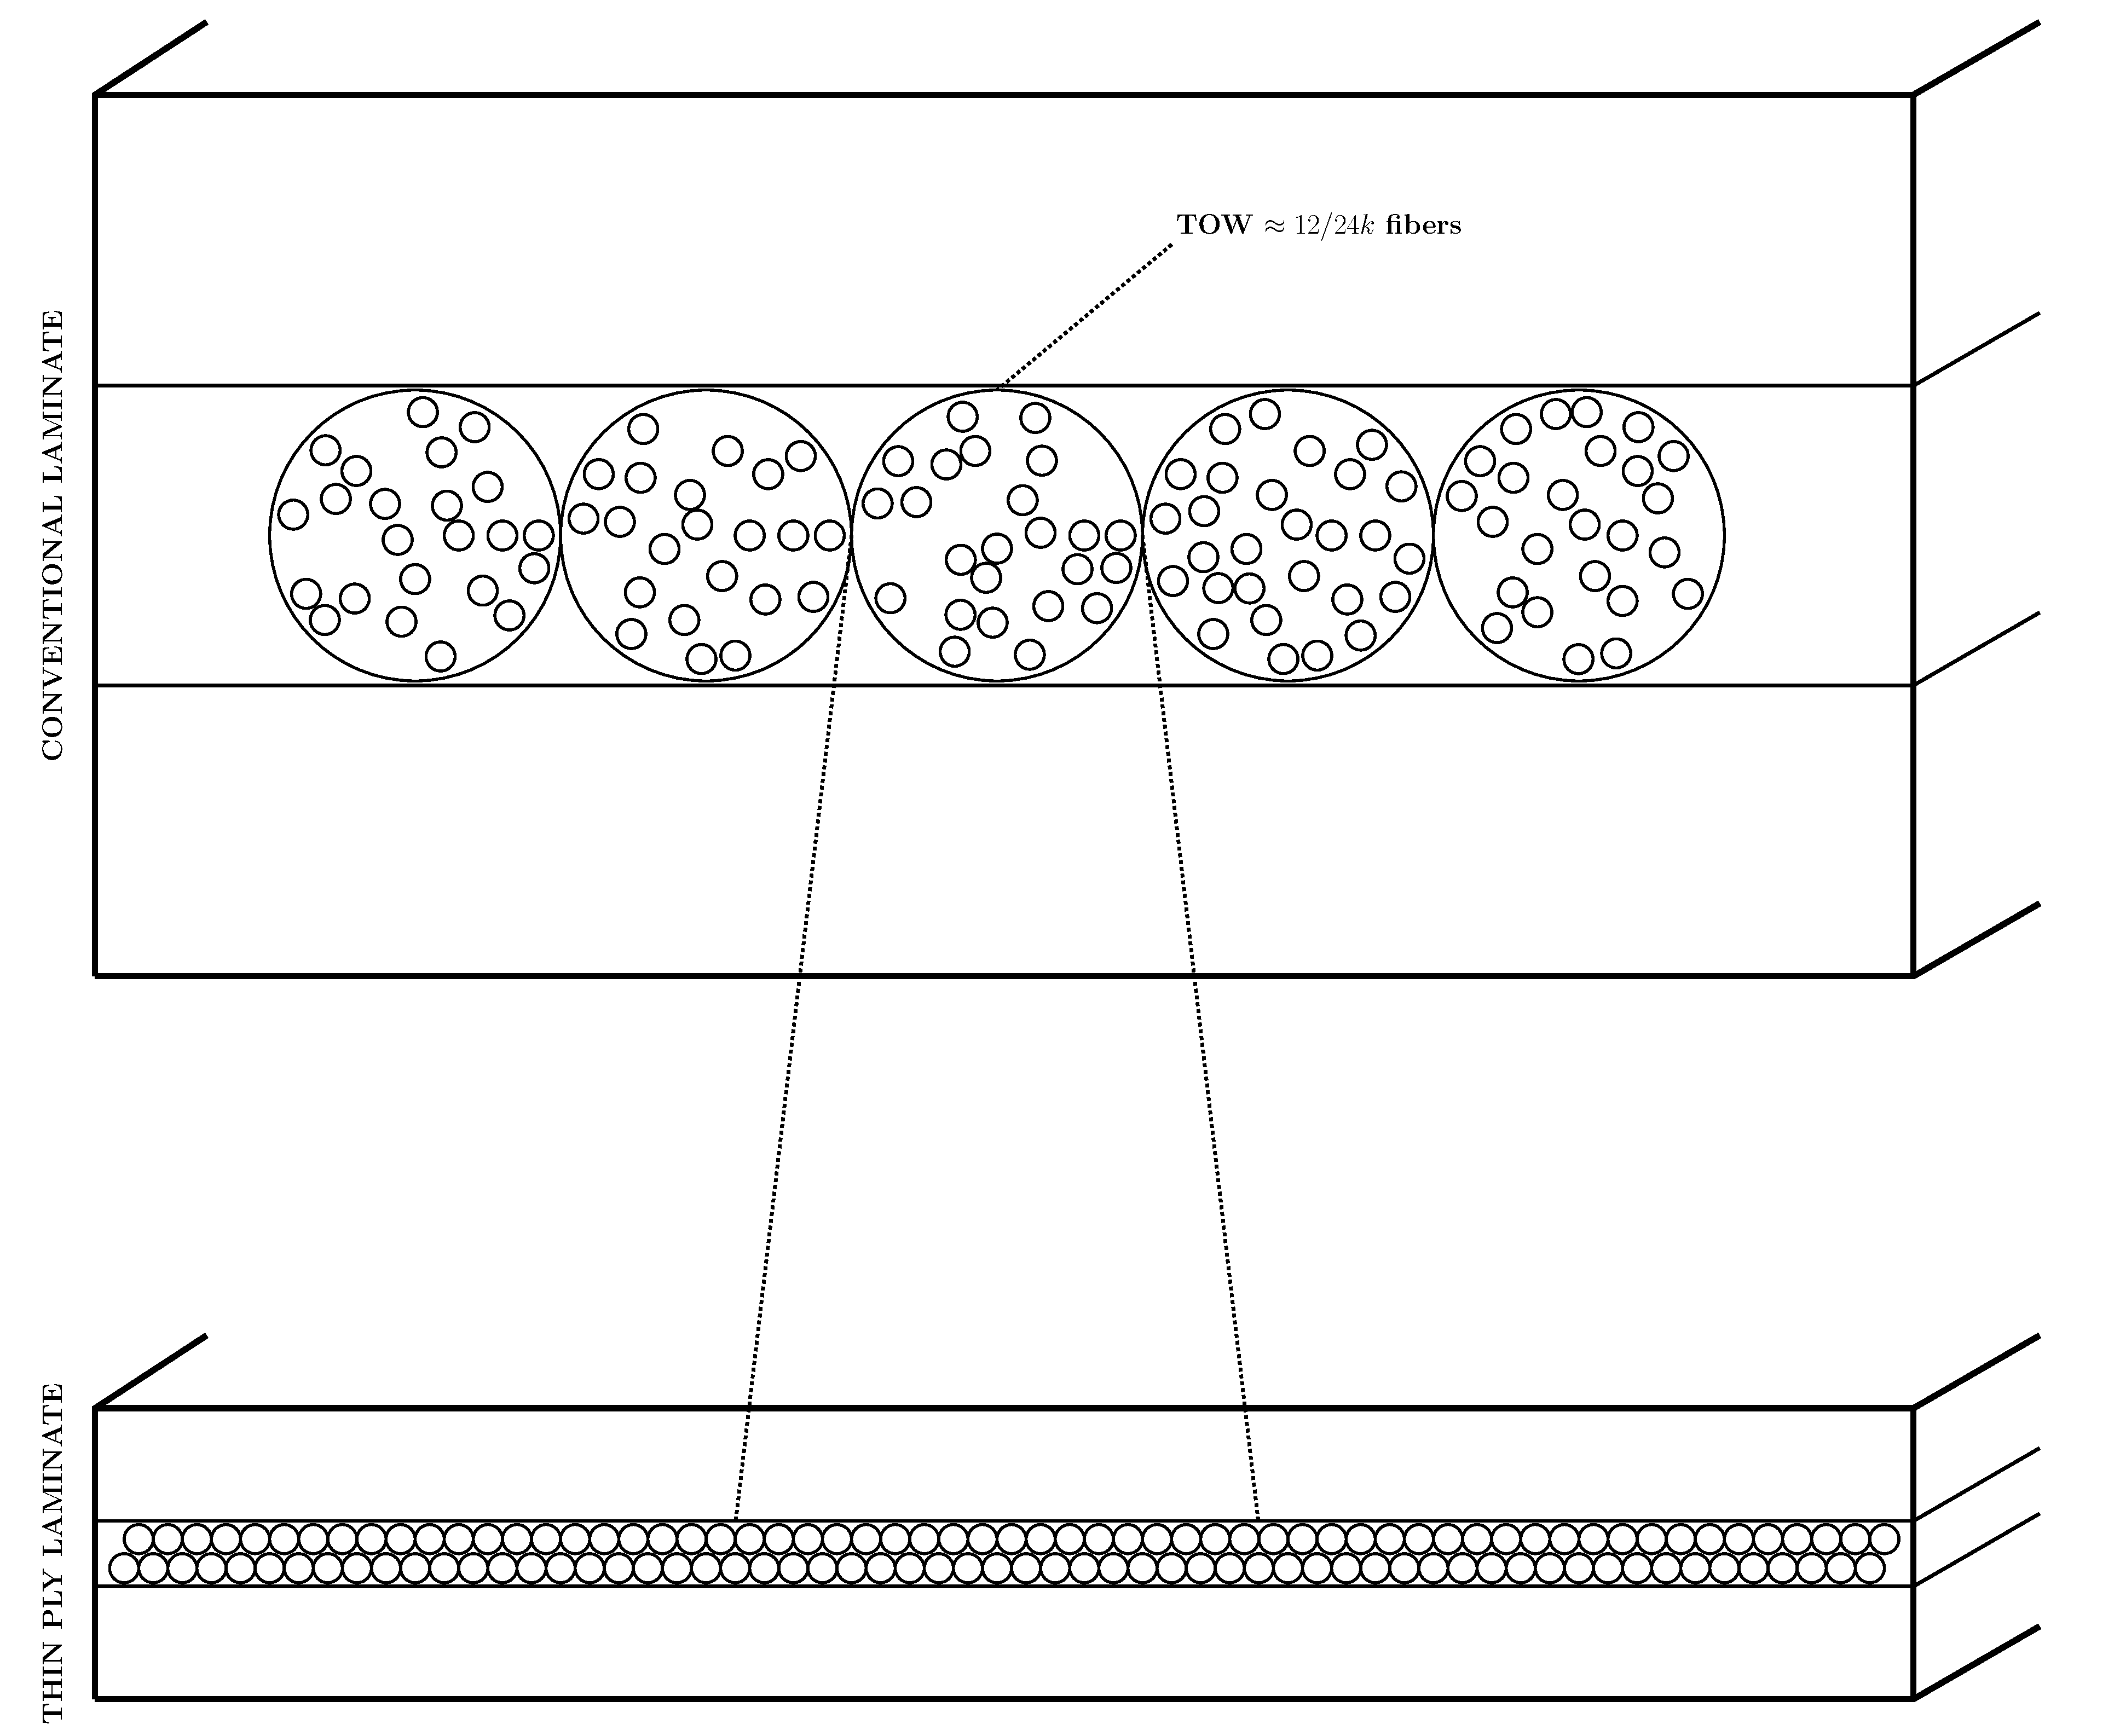
\includegraphics[width=0.75\columnwidth,height=0.125\textheight]{spread-tow-tech.pdf}}\\[40pt]
\subfloat[\small Solar Impulse 2, from {[}1{]}.]{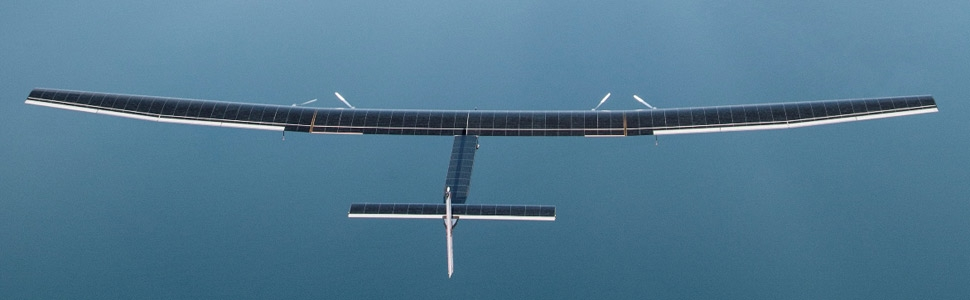
\includegraphics[width=0.45\columnwidth,height=0.04\textheight]{ntpt_solar-impulse-1.jpg}}\quad
\subfloat[\small Nuon Solar team's car, from {[}2{]}.]{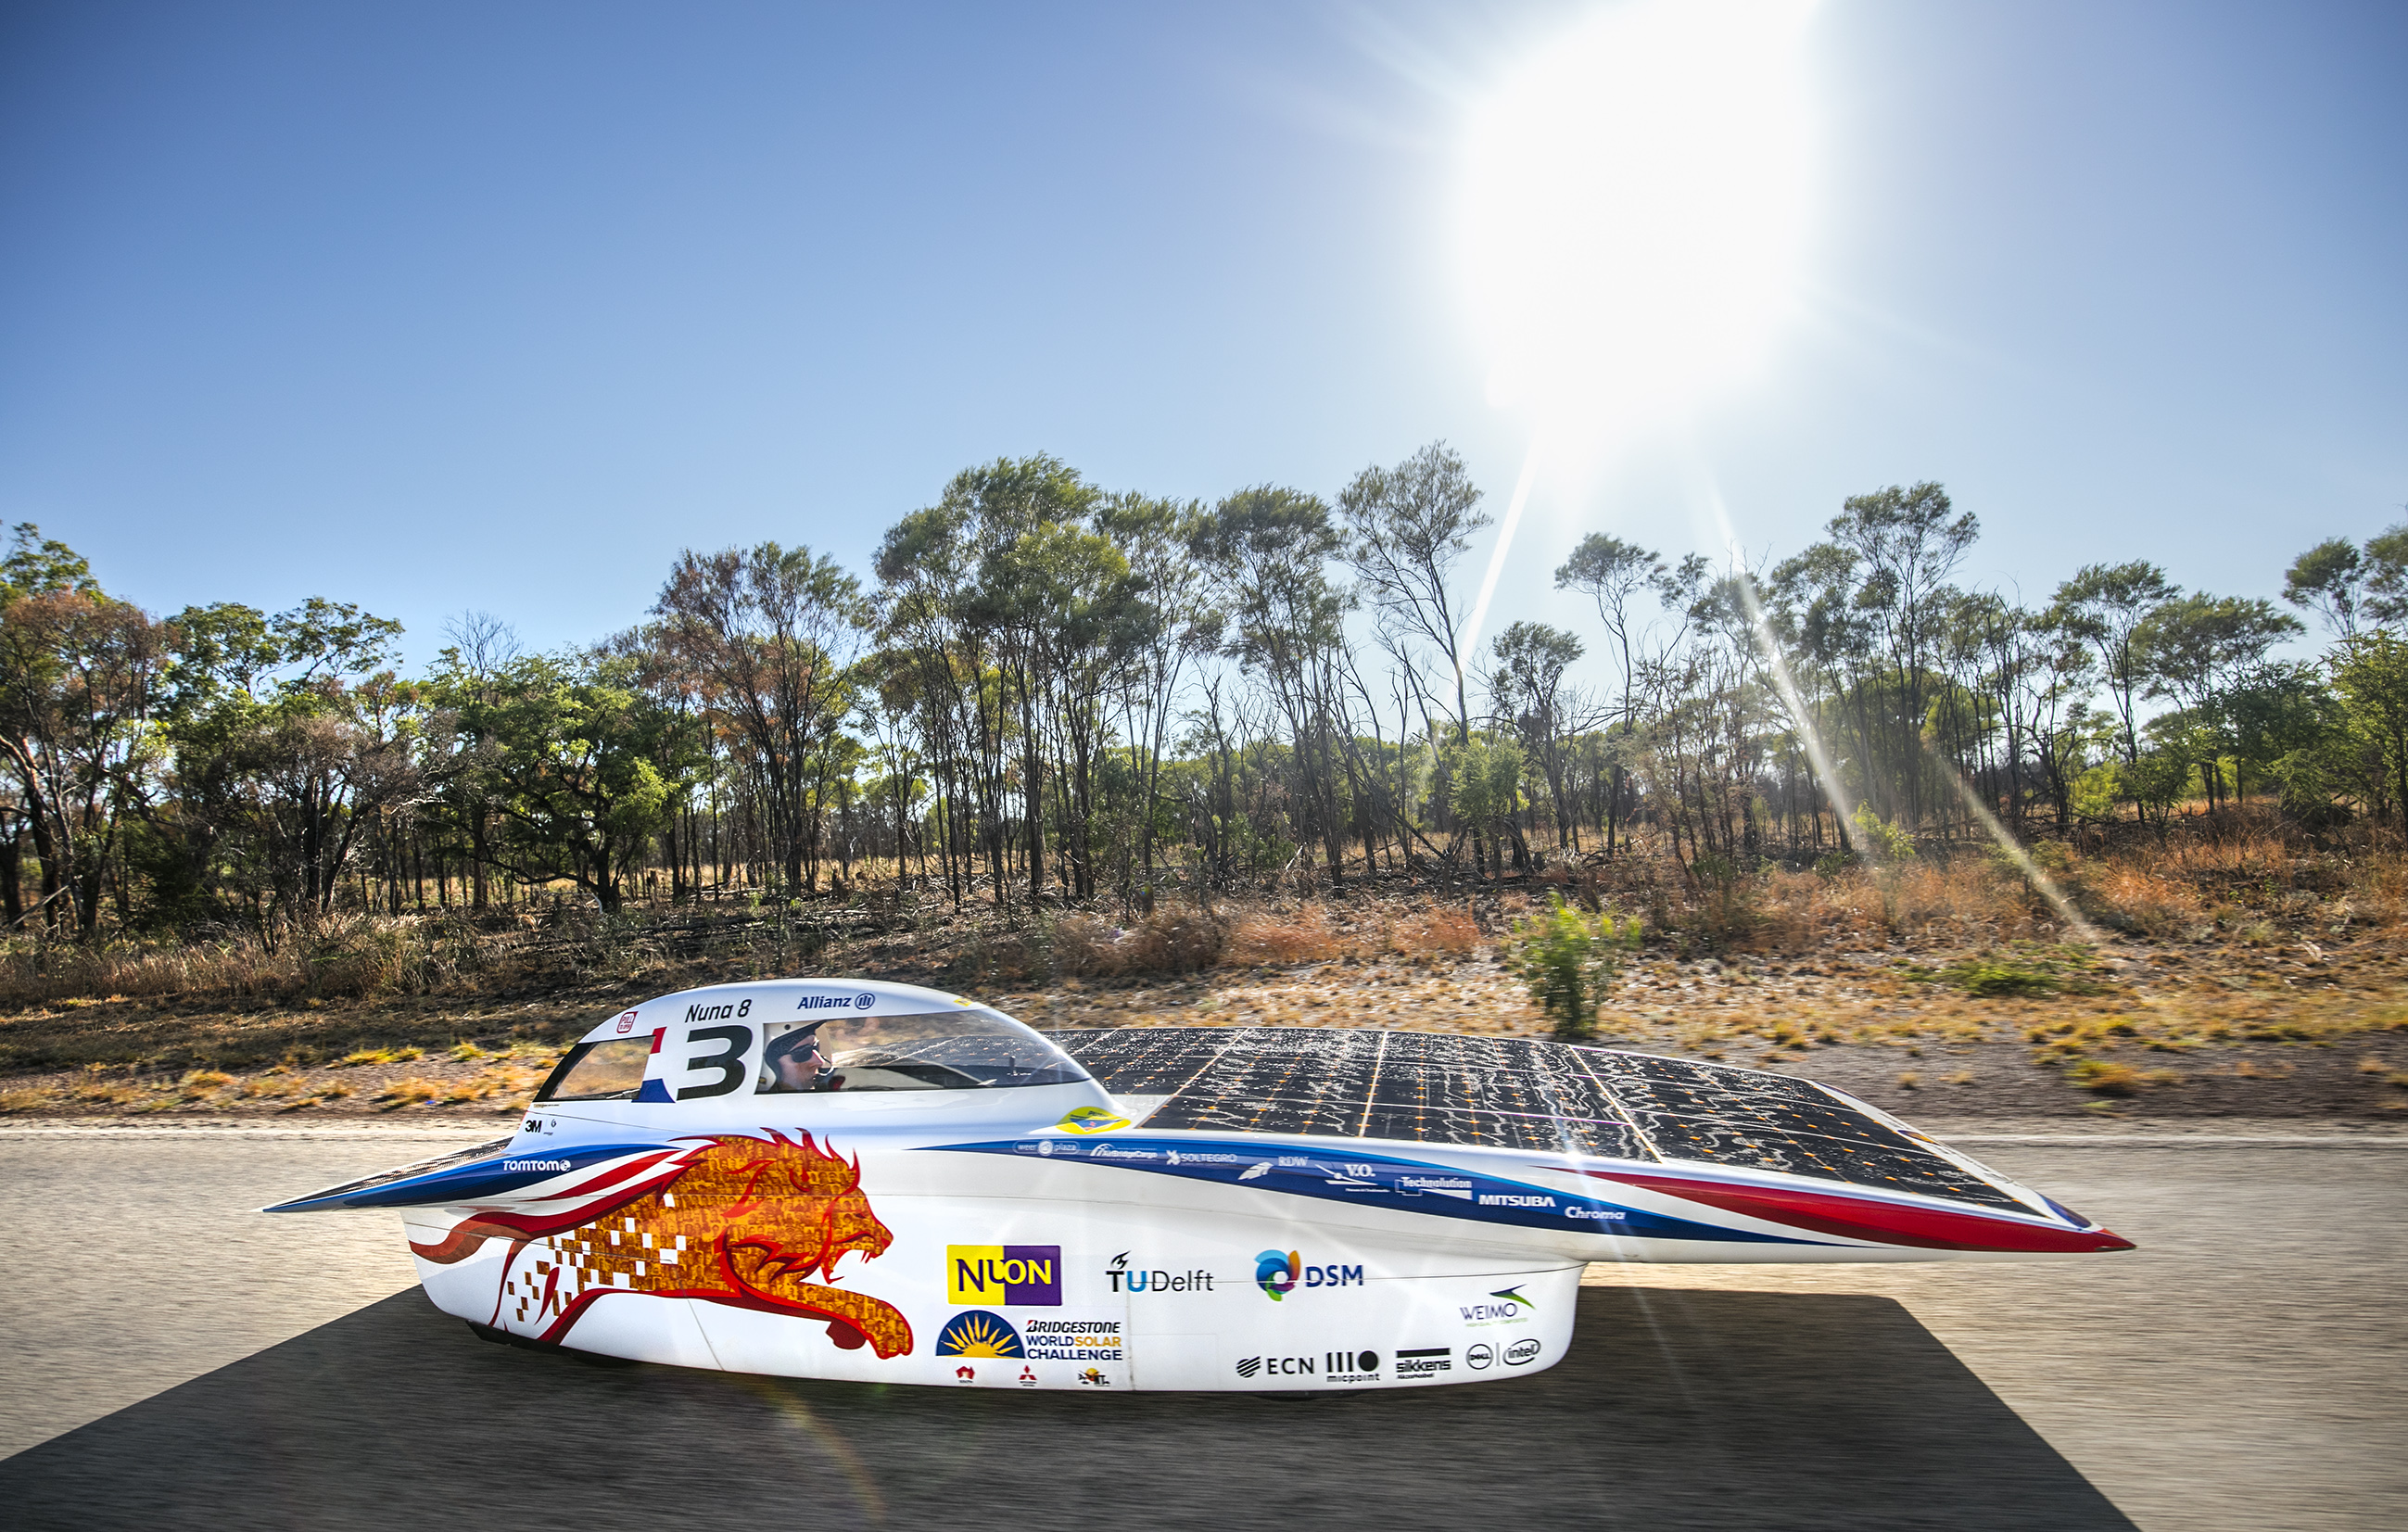
\includegraphics[width=0.45\columnwidth,height=0.04\textheight]{textreme_solar_car.jpg}}
\end{figure}
\end{center}
\end{column}
\begin{column}{0.25\textwidth}  %%<--- here
  \begin{center}
\textbf{Damage in FRPCs: a visual introduction}
\captionsetup[subfigure]{labelformat=empty}
\begin{figure}[!h]
\centering
     \subfloat[\small By Dr. R. Olsson, Swerea, SE.\label{fig:all-cracks}]{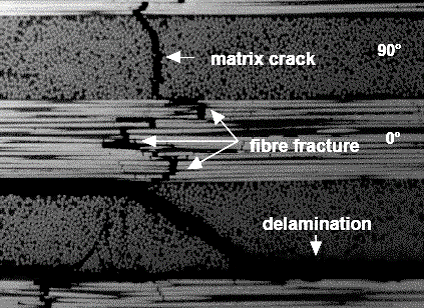
\includegraphics[width=0.75\columnwidth,height=0.09\textheight]{all-cracks.png}}\\
\subfloat[\small By Prof. Dr. E. K. Gamstedt, KTH, SE.\label{fig:transverse-cracks}]{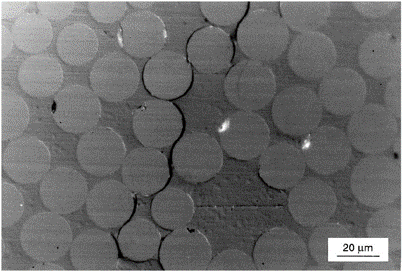
\includegraphics[width=0.75\columnwidth,height=0.09\textheight]{intralaminar-cracks.png}}
\end{figure}
     \end{center}
\end{column}
\begin{column}{0.35\textwidth}  %%<--- here
    \begin{center}
\textbf{The thin ply effect}

\begin{figure}[!h]
\centering
     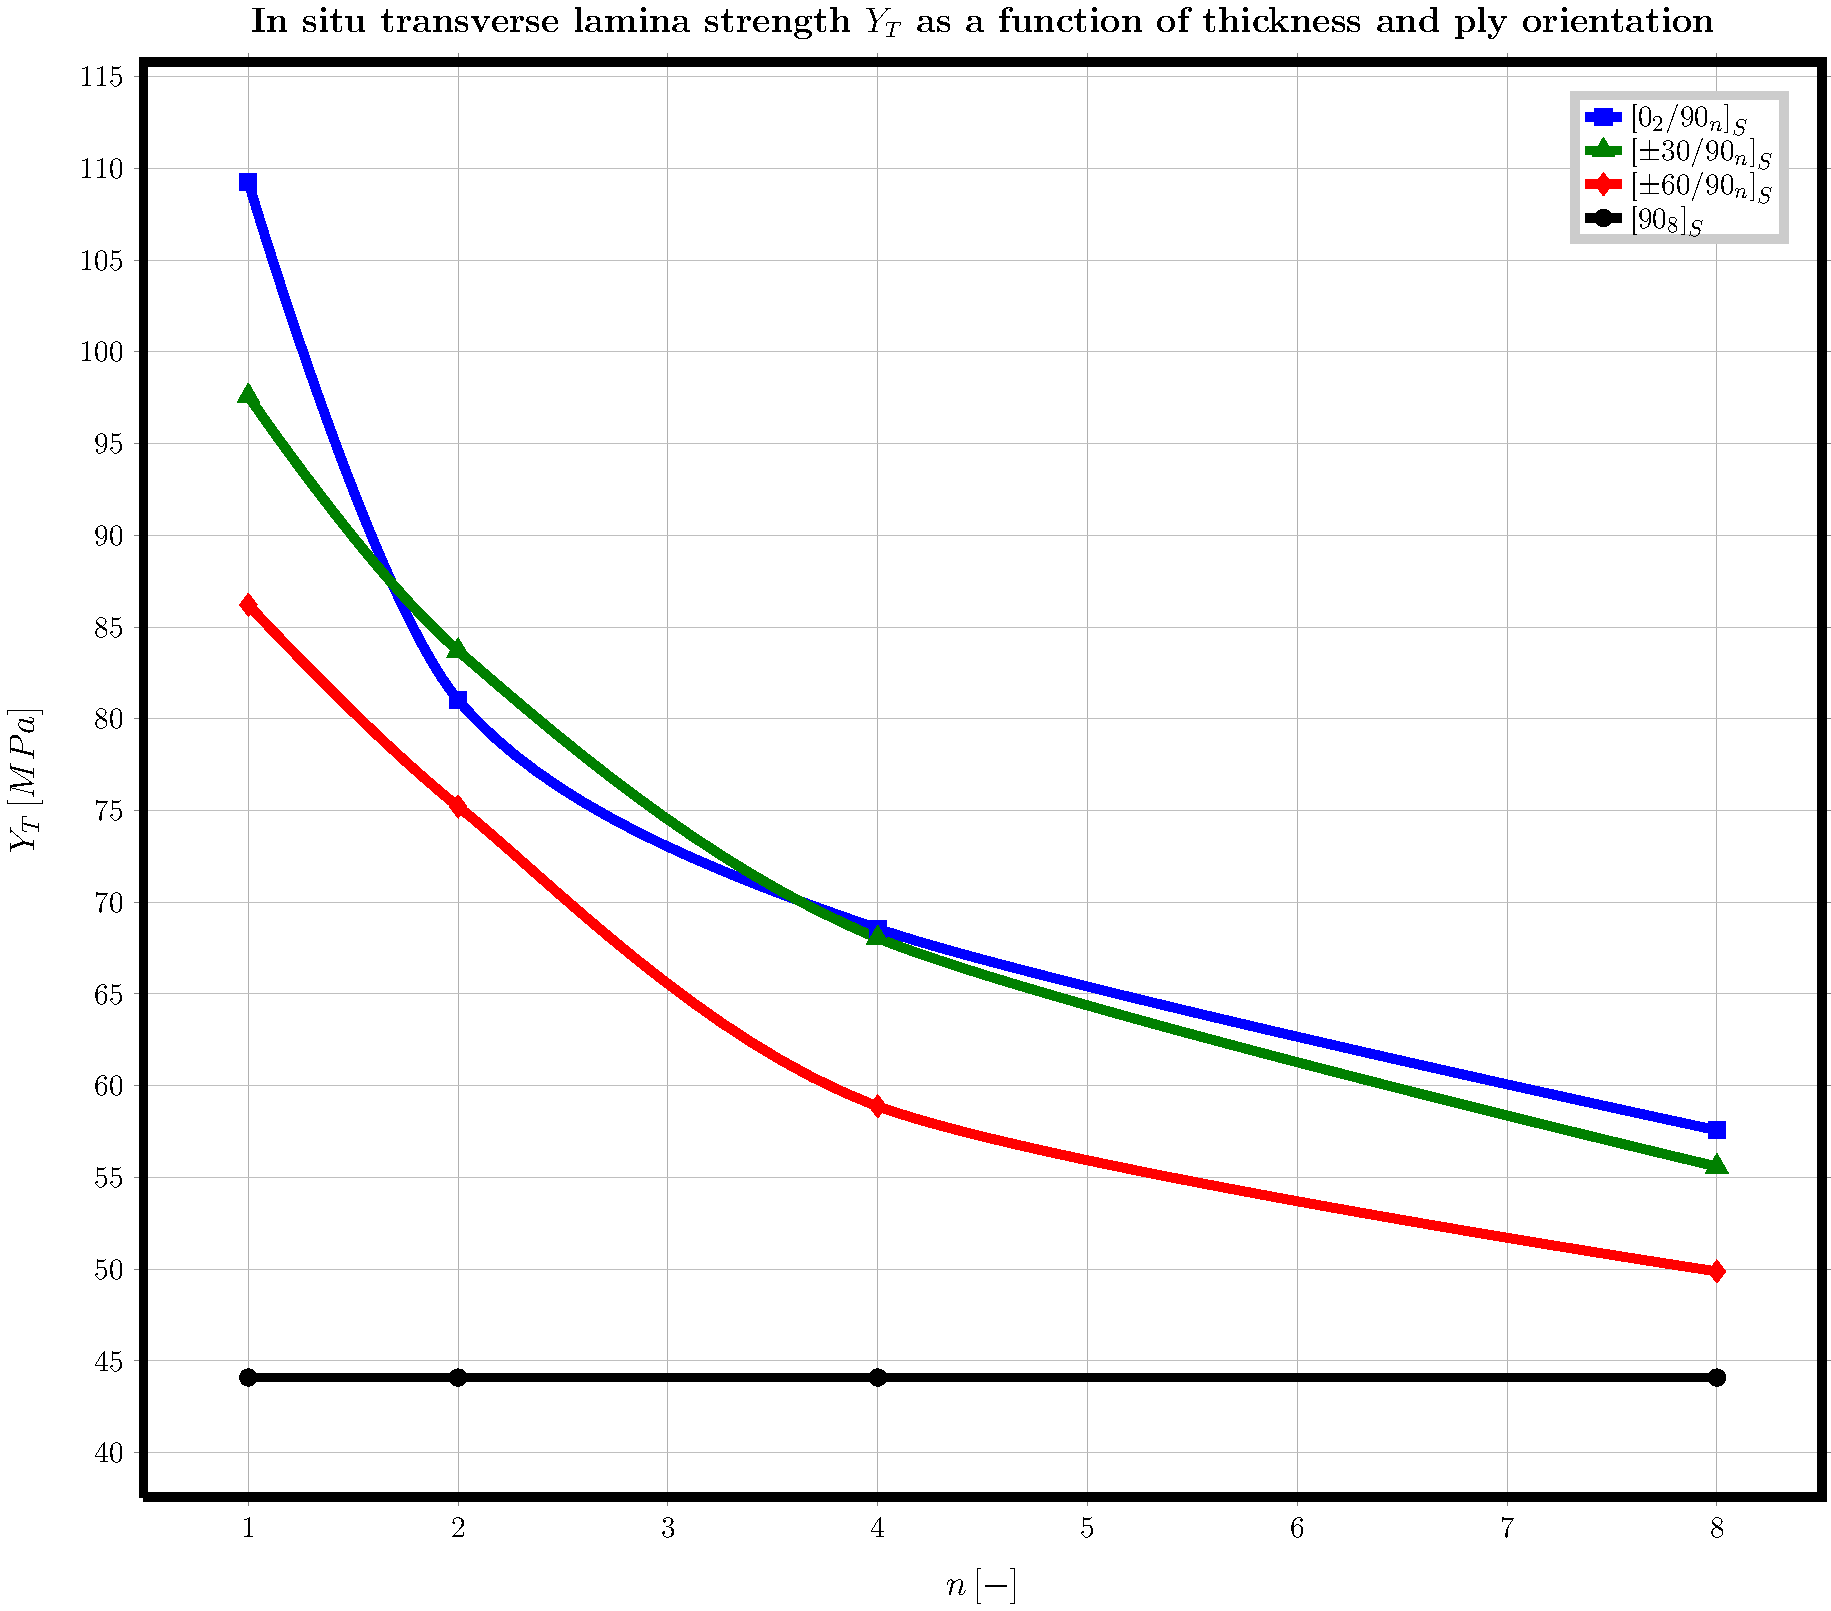
\includegraphics[width=0.9\columnwidth,height=0.175\textheight]{Flaggs-Kural_InSituTransverseStrength.pdf}
\caption{\small Measurements of in-situ transverse strength from Flaggs \& Kural, 1982 [3].}
\end{figure}
     \end{center}
\end{column}
\end{columns}
%\begin{figure}[!h]
%\centering
%\subfloat[\scriptsize By Dr. R. Olsson, Swerea, SE.\label{fig:all-cracks}]{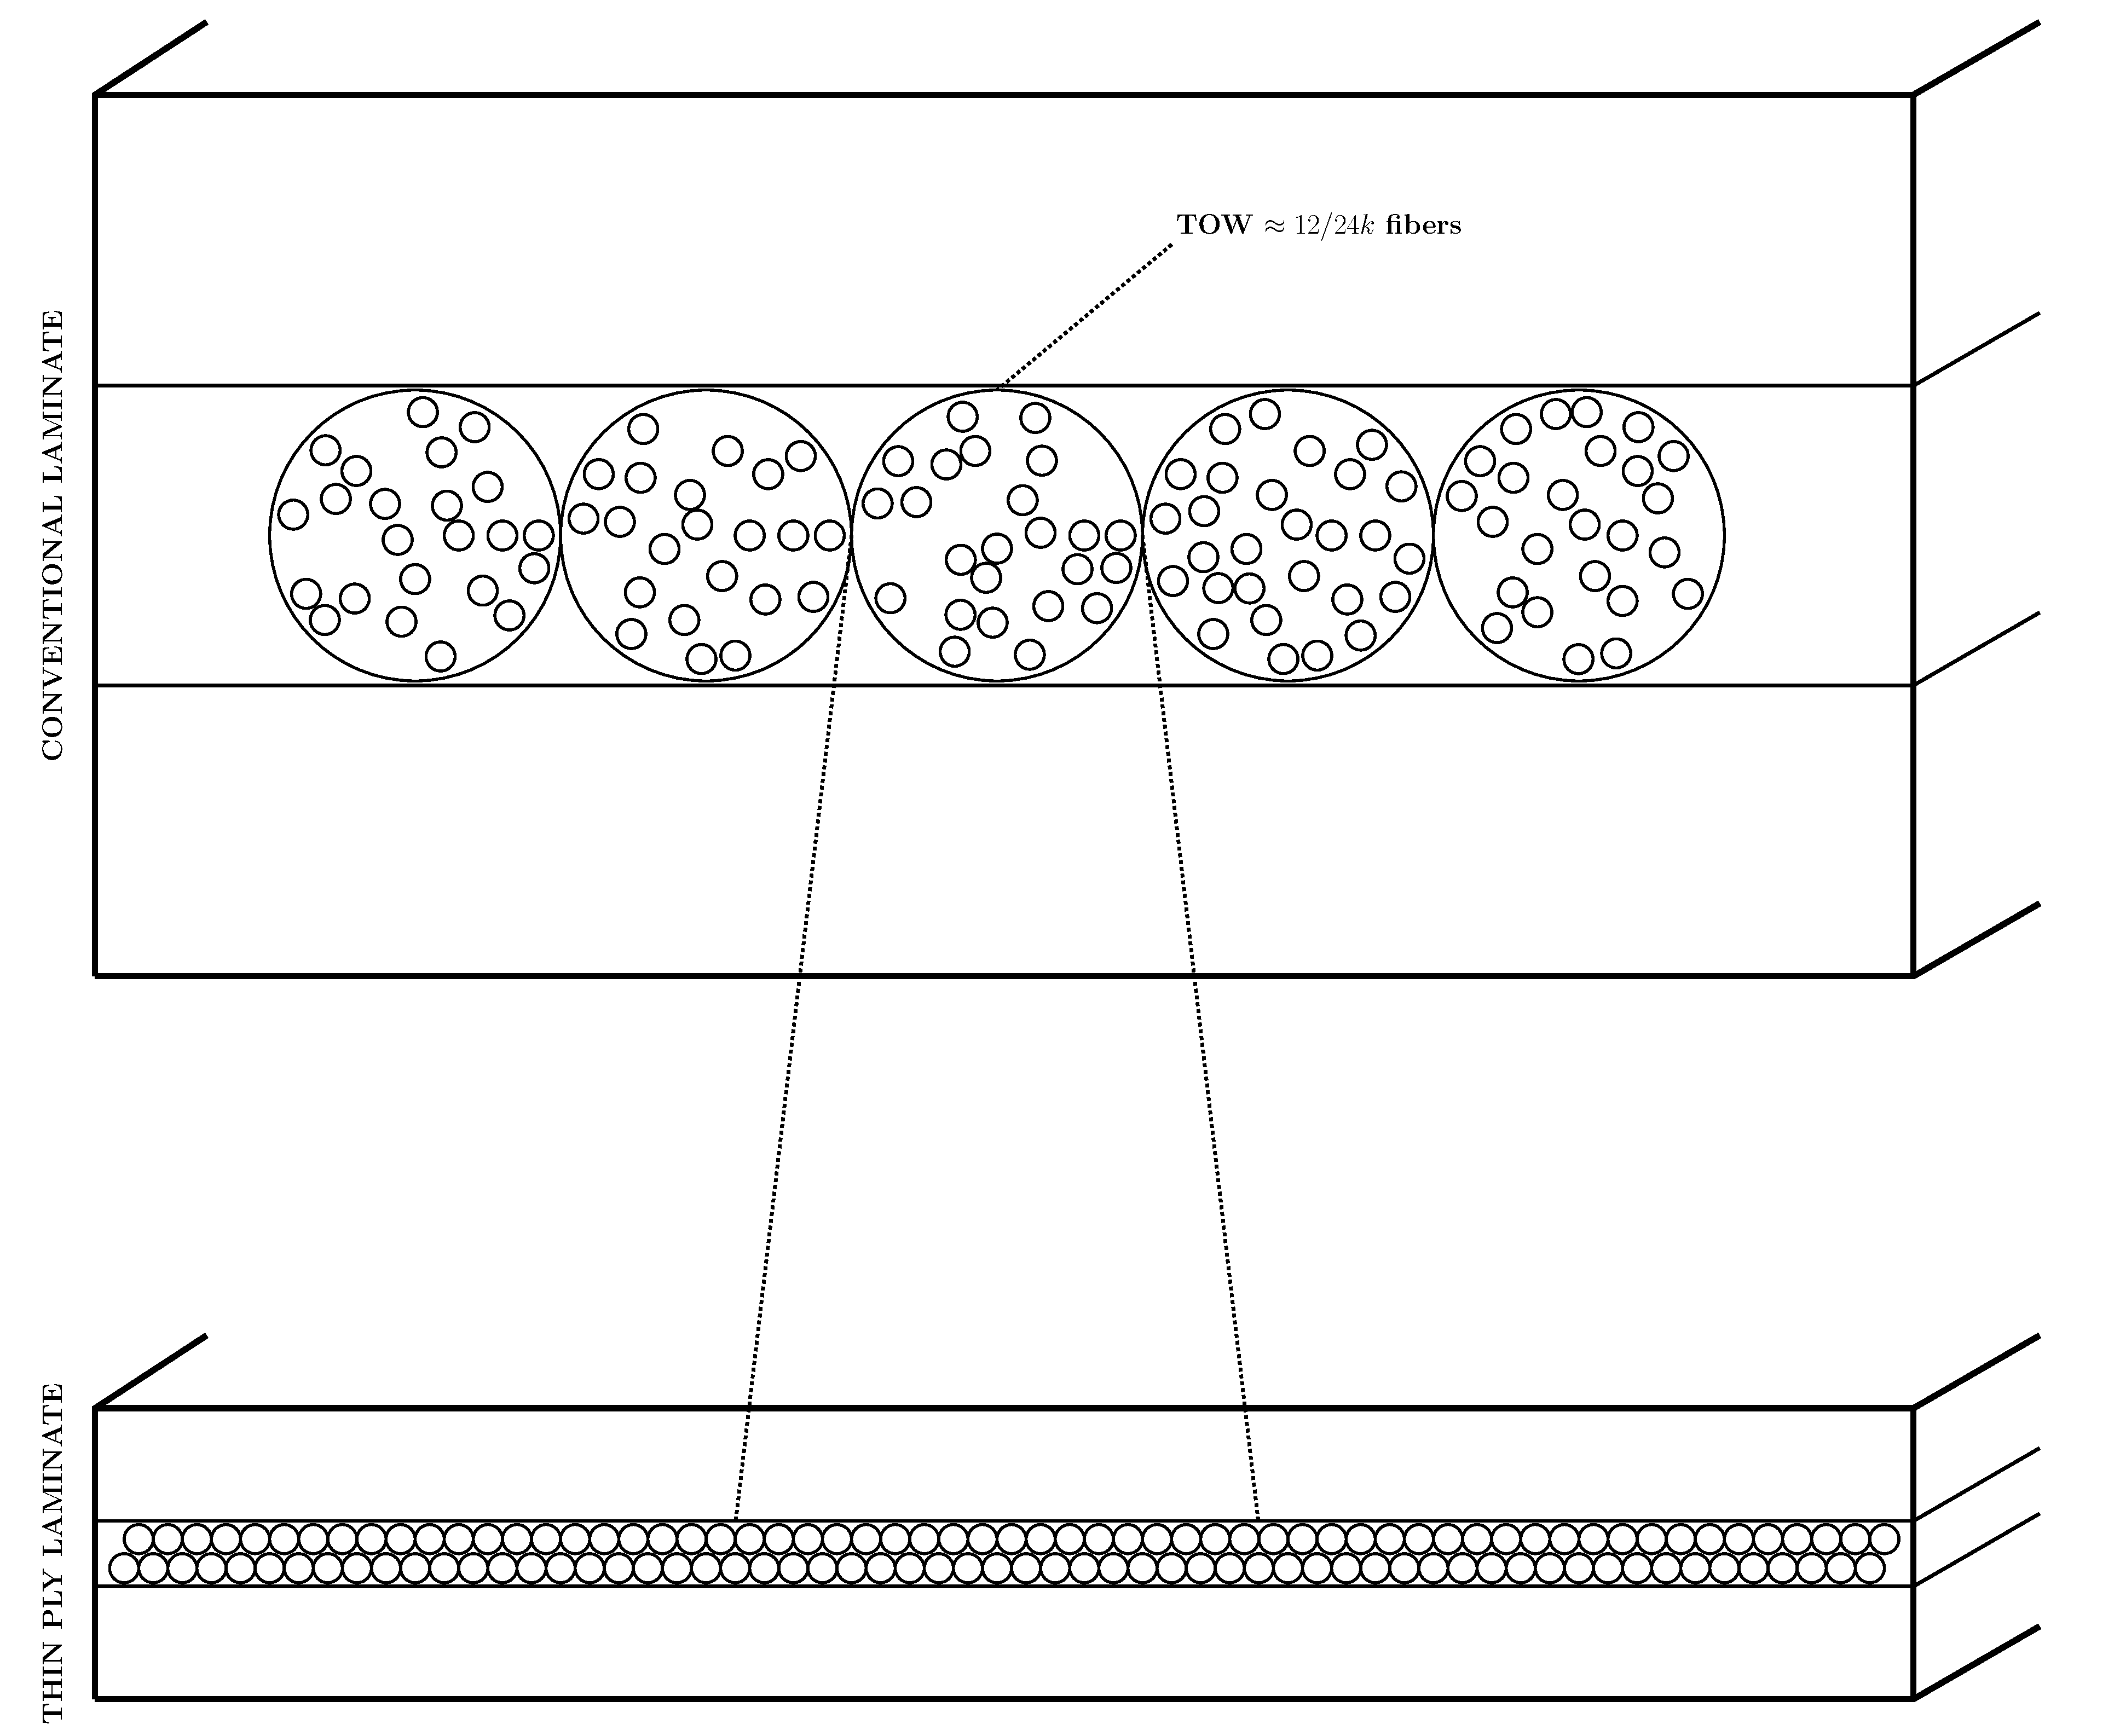
\includegraphics[width=0.25\textwidth]{spread-tow-tech.pdf}}\quad
%\subfloat[\scriptsize By Dr. R. Olsson, Swerea, SE.\label{fig:all-cracks}]{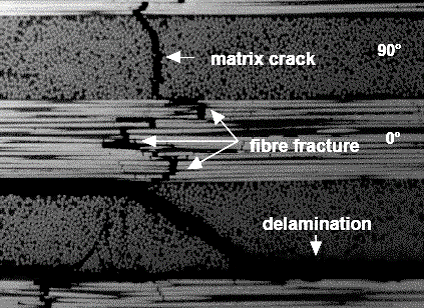
\includegraphics[width=0.25\textwidth]{all-cracks.png}}\quad
%\subfloat[\scriptsize By Prof. Dr. E. K. Gamstedt, KTH, SE.\label{fig:transverse-cracks}]{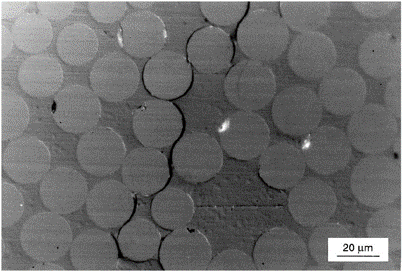
\includegraphics[width=0.25\textwidth]{intralaminar-cracks.png}}\quad
%\subfloat[\scriptsize By Prof. Dr. E. K. Gamstedt, KTH, SE.\label{fig:transverse-cracks}]{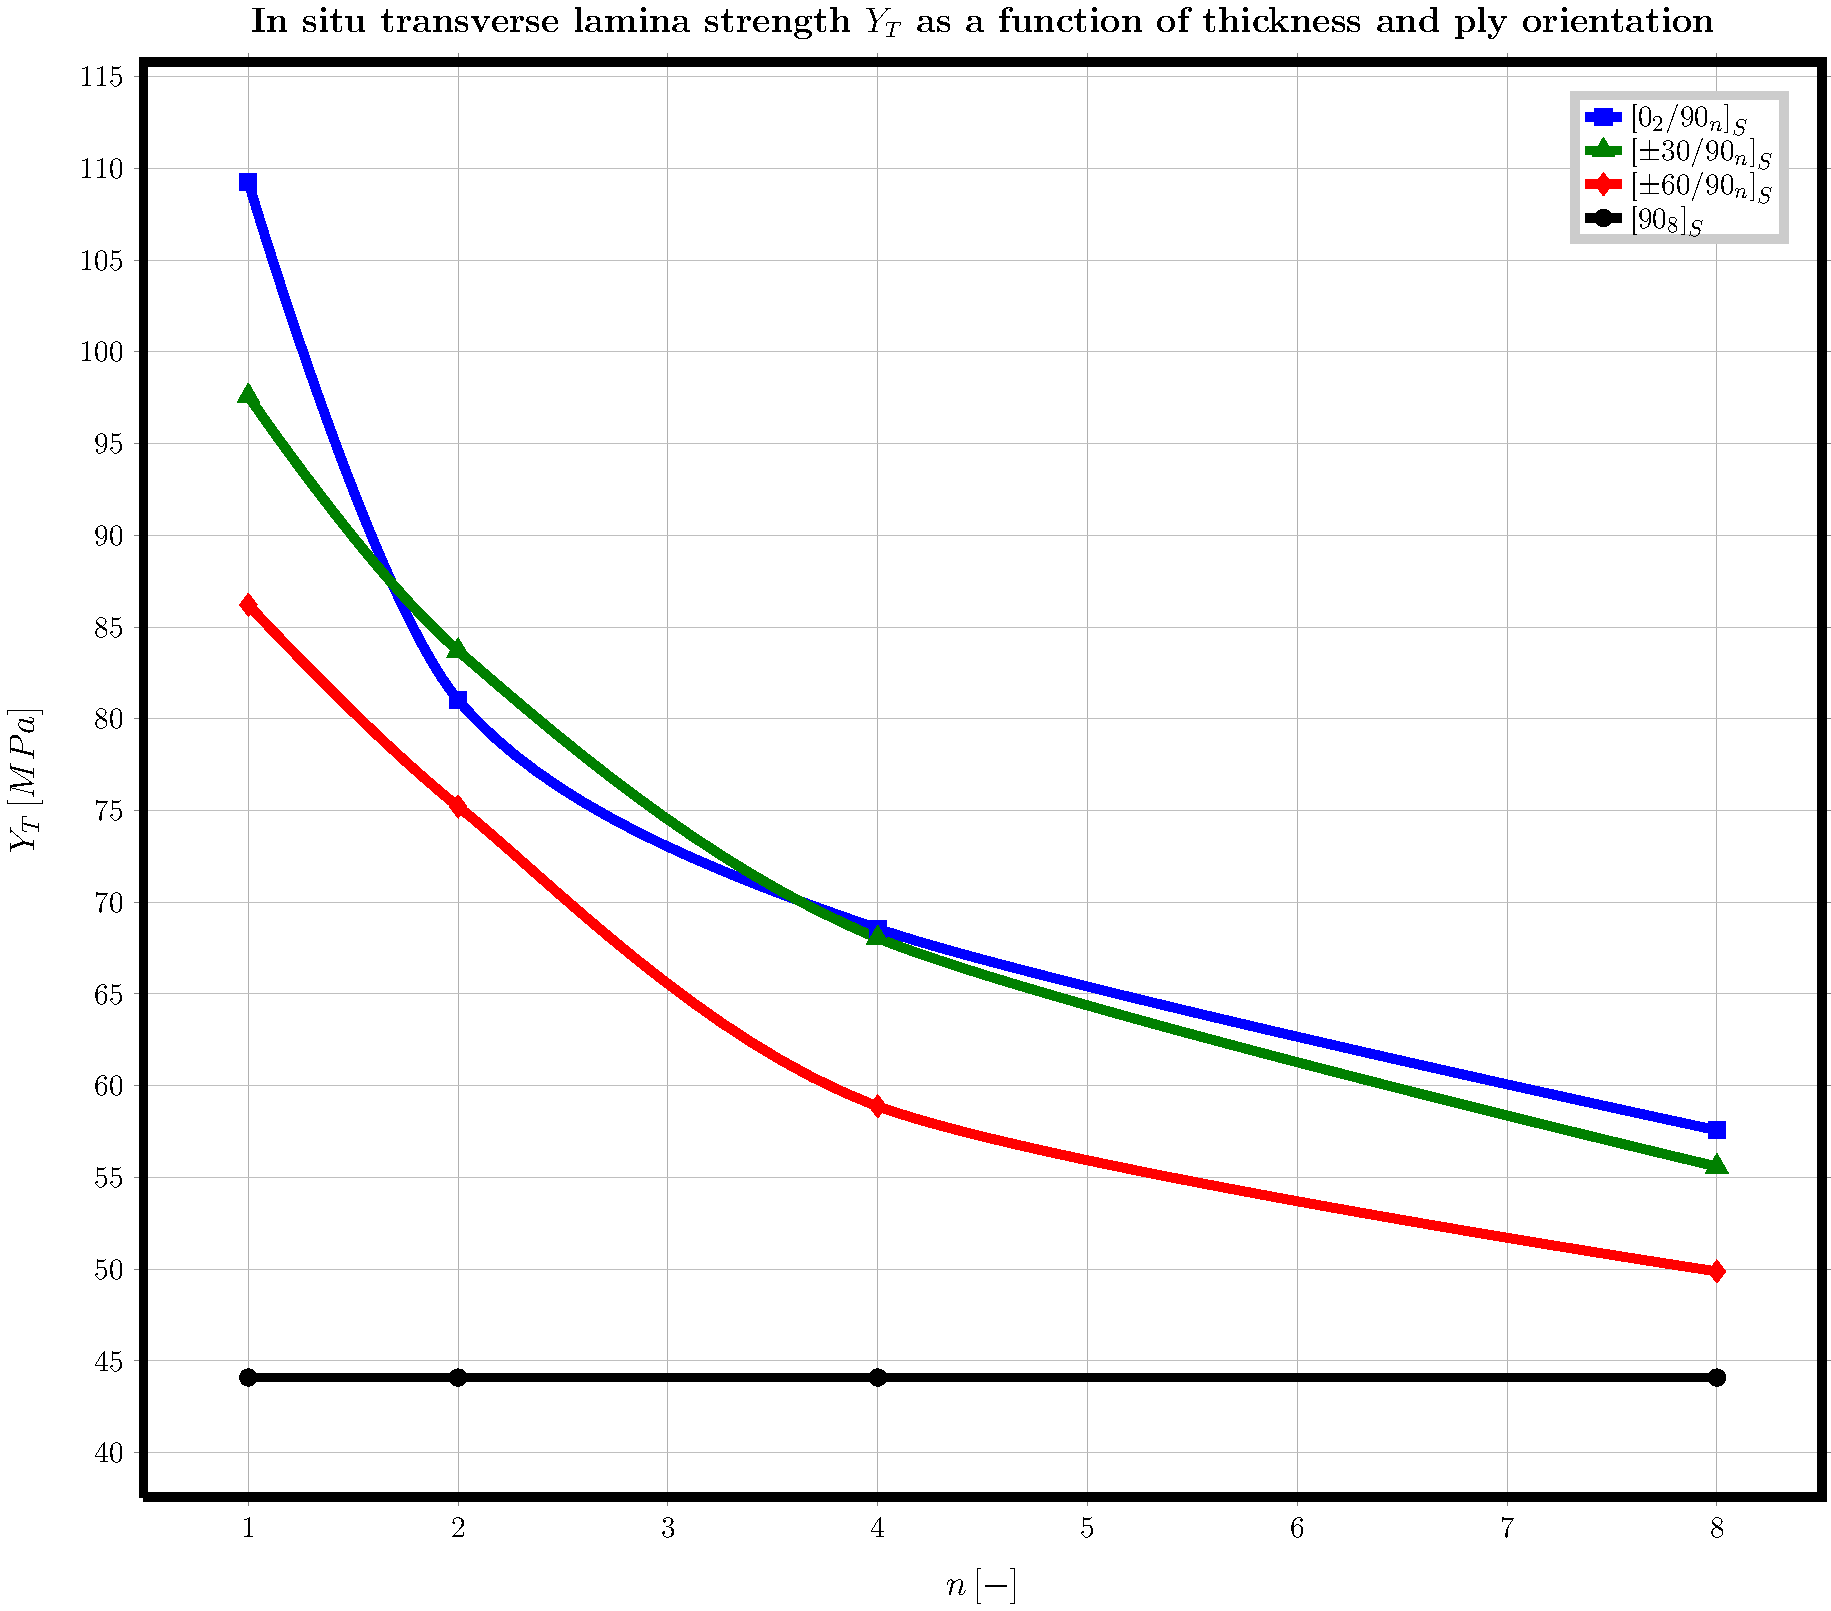
\includegraphics[width=0.25\textwidth]{Flaggs-Kural_InSituTransverseStrength.pdf}}
% \caption{For a visual definition of intralaminar transverse cracking.}
%  \label{fig:intralaminar-cracks}
%\end{figure}
\end{block}
\end{minipage}
\end{center}

\begin{center}
	\begin{minipage}{\textwidth}
		\begin{alertblock}{\rule[-0.6ex]{0pt}{50pt}\centering\LARGE Objectives \& Approach}
			\begin{columns}
				\begin{column}{0.475\textwidth}
   					 \begin{center}
						\textbf{What do we want to achieve?}\\[5pt]
							\begin{itemize}
    								\item Investigate the influence of volume fraction, material properties, thin ply thickness and bounding plies' thicknesses on crack initiation\\[10pt]
    								\item $G_{*c}=G_{*c}\left(\theta_{debond},\Delta\theta_{debond}, E_{\left(\cdot\cdot\right)}, \nu_{\left(\cdot\cdot\right)}, G_{\left(\right)},VF_{f}, t_{ply}, \frac{t_{ply}}{t_{bounding\ plies}}\right)$
							\end{itemize}
   					\end{center}
				\end{column}
				\begin{column}{0.475\textwidth}  %%<--- here
   					\begin{center}
						\textbf{How do we want to achieve it?}\\[5pt]
						\begin{itemize}
    							\item Design and categorization of several Representative Volume Elements (RVEs)
    							\item Automated generation of RVEs geometry and FEM model
    							\item Finite Element Simulations (in Abaqus)
						\end{itemize}
   					\end{center}
				\end{column}
			\end{columns}
		\end{alertblock}
	\end{minipage}
\end{center}



\begin{center}
\begin{minipage}{\textwidth}
\begin{exampleblock}{\rule[-0.6ex]{0pt}{50pt}\centering\LARGE Design \& Analysis of Representative Volume Elements (RVEs)}
\begin{columns}
\begin{column}{0.3\textwidth}
\begin{center}
\begin{figure}[!h]
\centering
   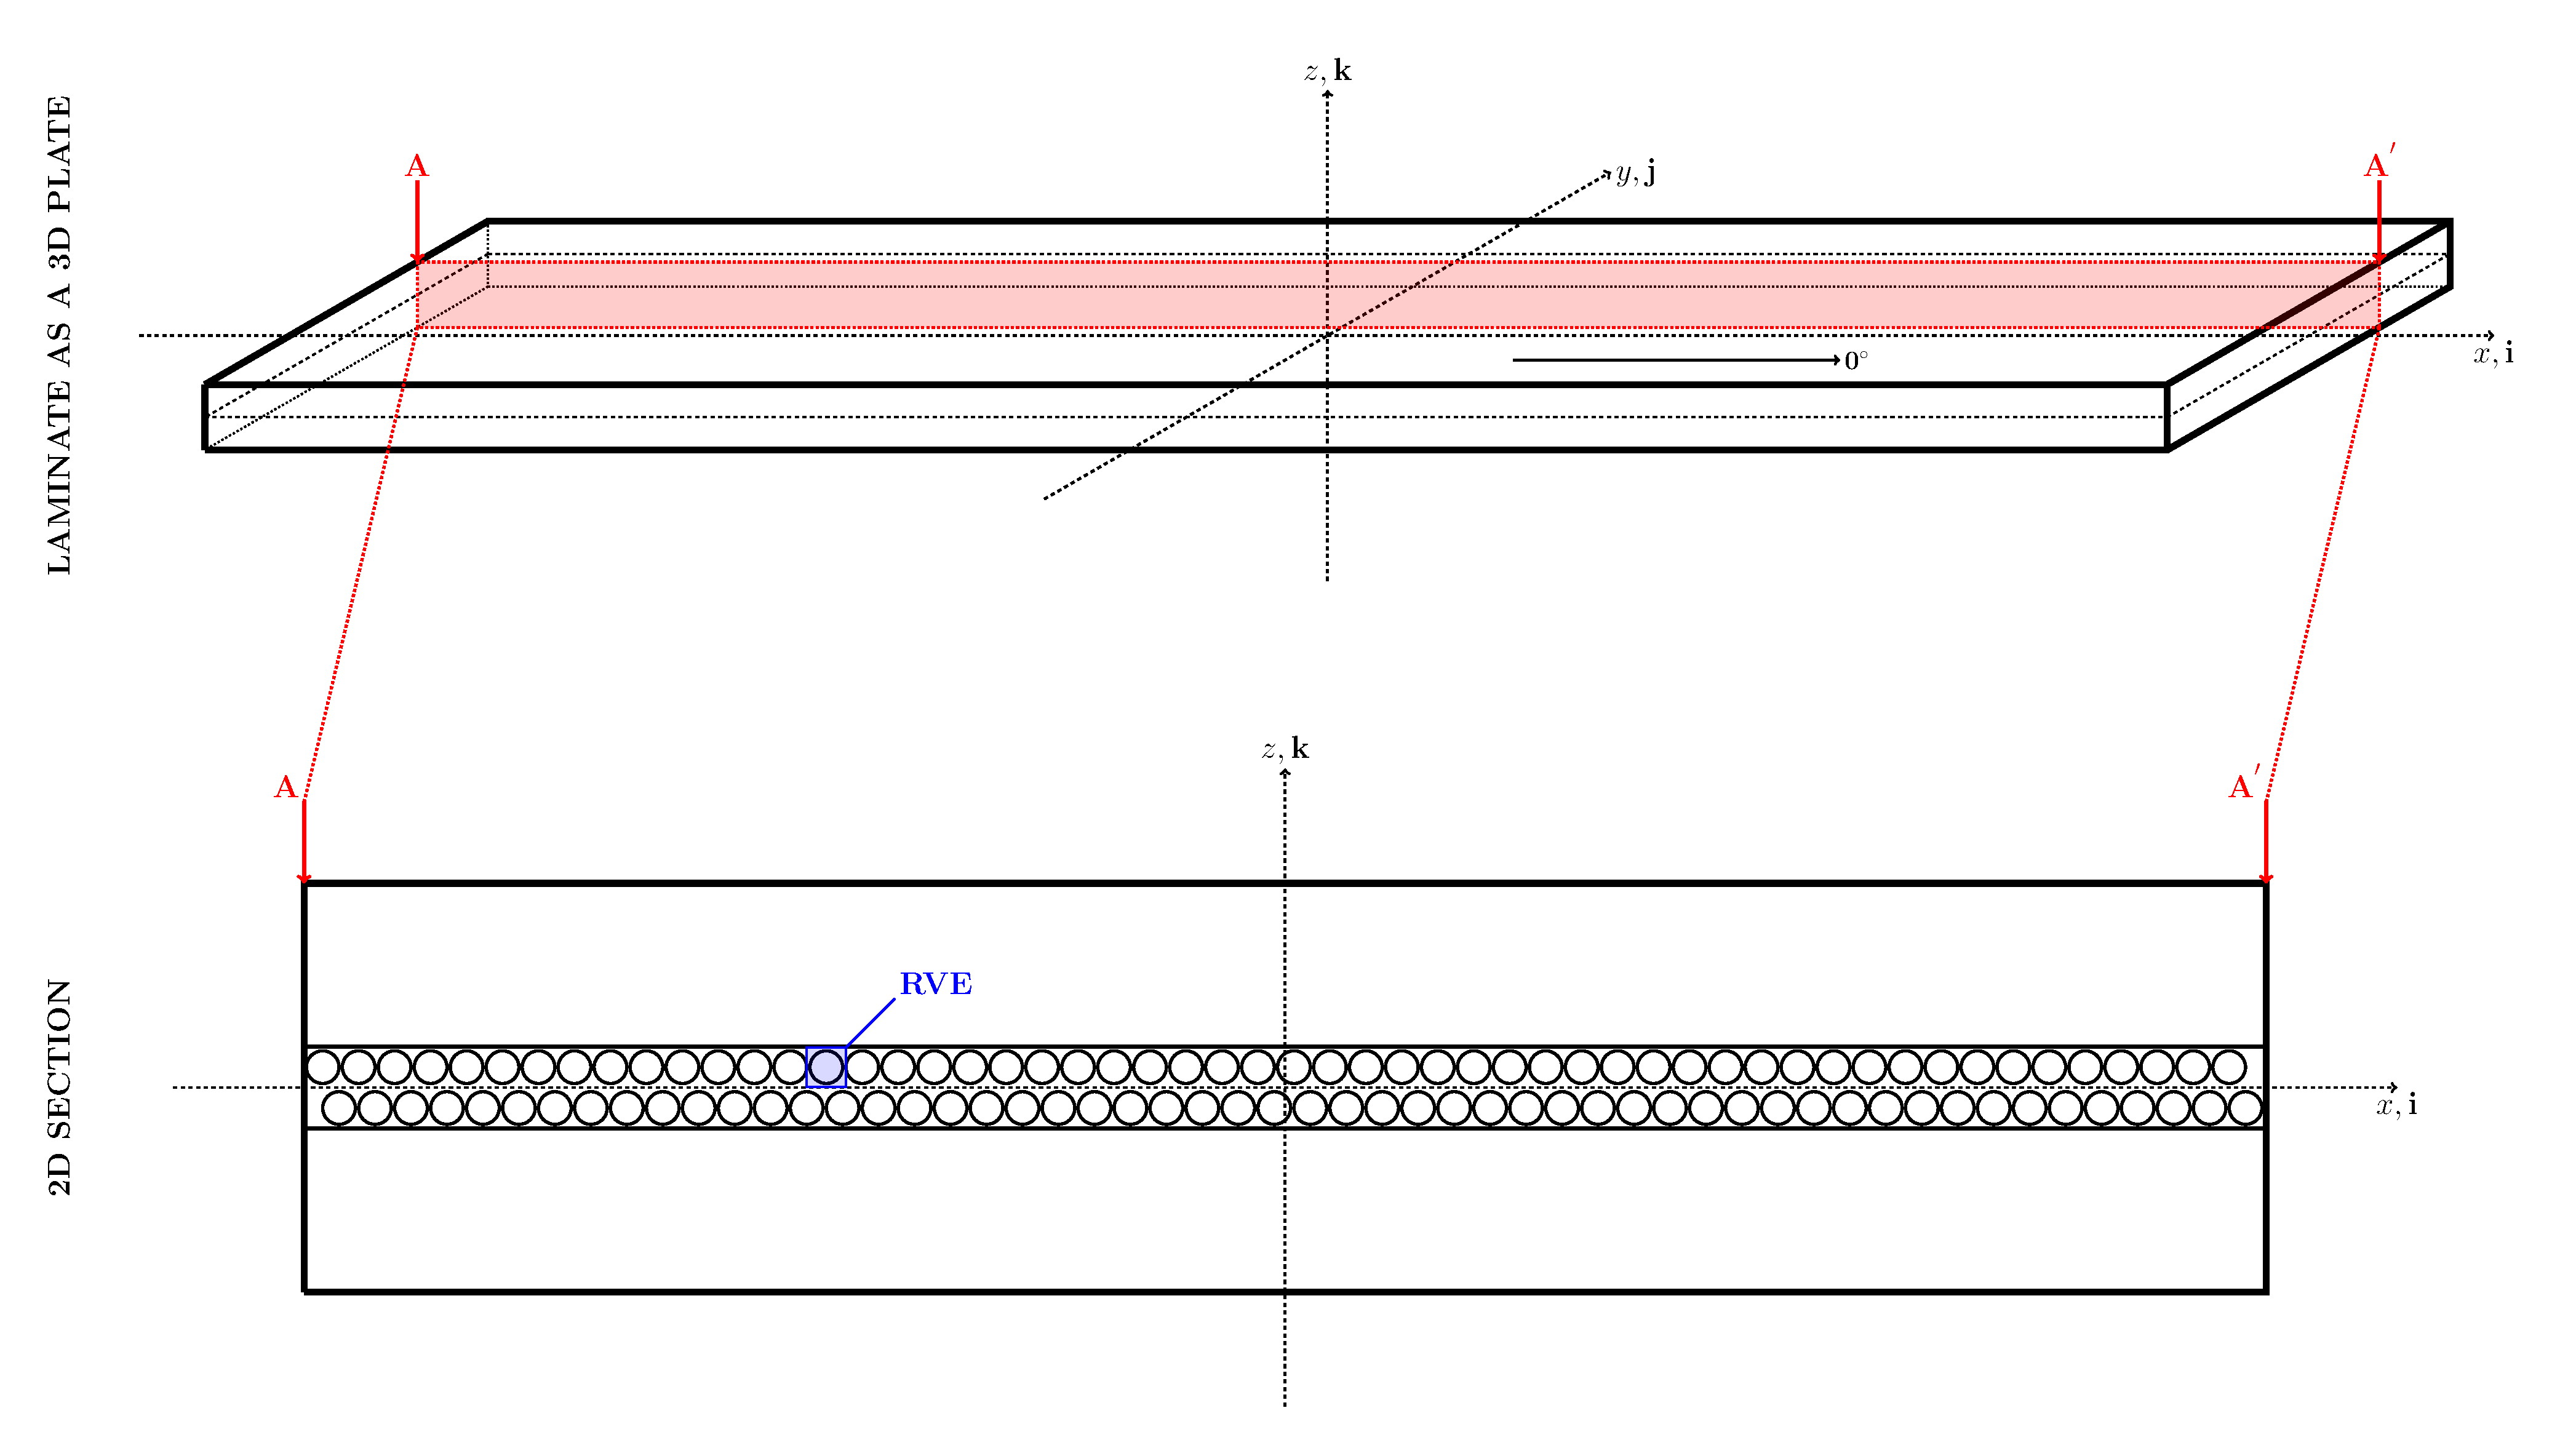
\includegraphics[width=\columnwidth]{laminate-section.pdf}
\end{figure}
\begin{columns}
\begin{column}{0.25\columnwidth}
\end{column}
\begin{column}{0.5\columnwidth}
\begin{itemize}
\small
\item[$\color{blue}\checkmark$]2D space
\item[$\color{blue}\checkmark$]Linear elastic materials
\item[$\color{blue}\checkmark$]Displacement control
\item[$\color{blue}\checkmark$]Dirichlet-type boundary conditions
\item[$\color{blue}\checkmark$]Linear elastic fracture mechanics
\item[$\color{blue}\checkmark$]Contact interaction\\[5pt]
\end{itemize}
\end{column}
\begin{column}{0.25\columnwidth}
\end{column}
\end{columns}
\end{center}
\end{column}
\begin{column}{0.15\textwidth}  %%<--- here
    \begin{center}
\captionsetup[subfigure]{labelformat=empty}
\begin{figure}[!h]
\centering
\subfloat{\includegraphics[width=\columnwidth]{SingleRVEs.pdf}}
\end{figure}
     \end{center}
\end{column}
\begin{column}{0.125\textwidth}
\begin{figure}[!h]
\centering
   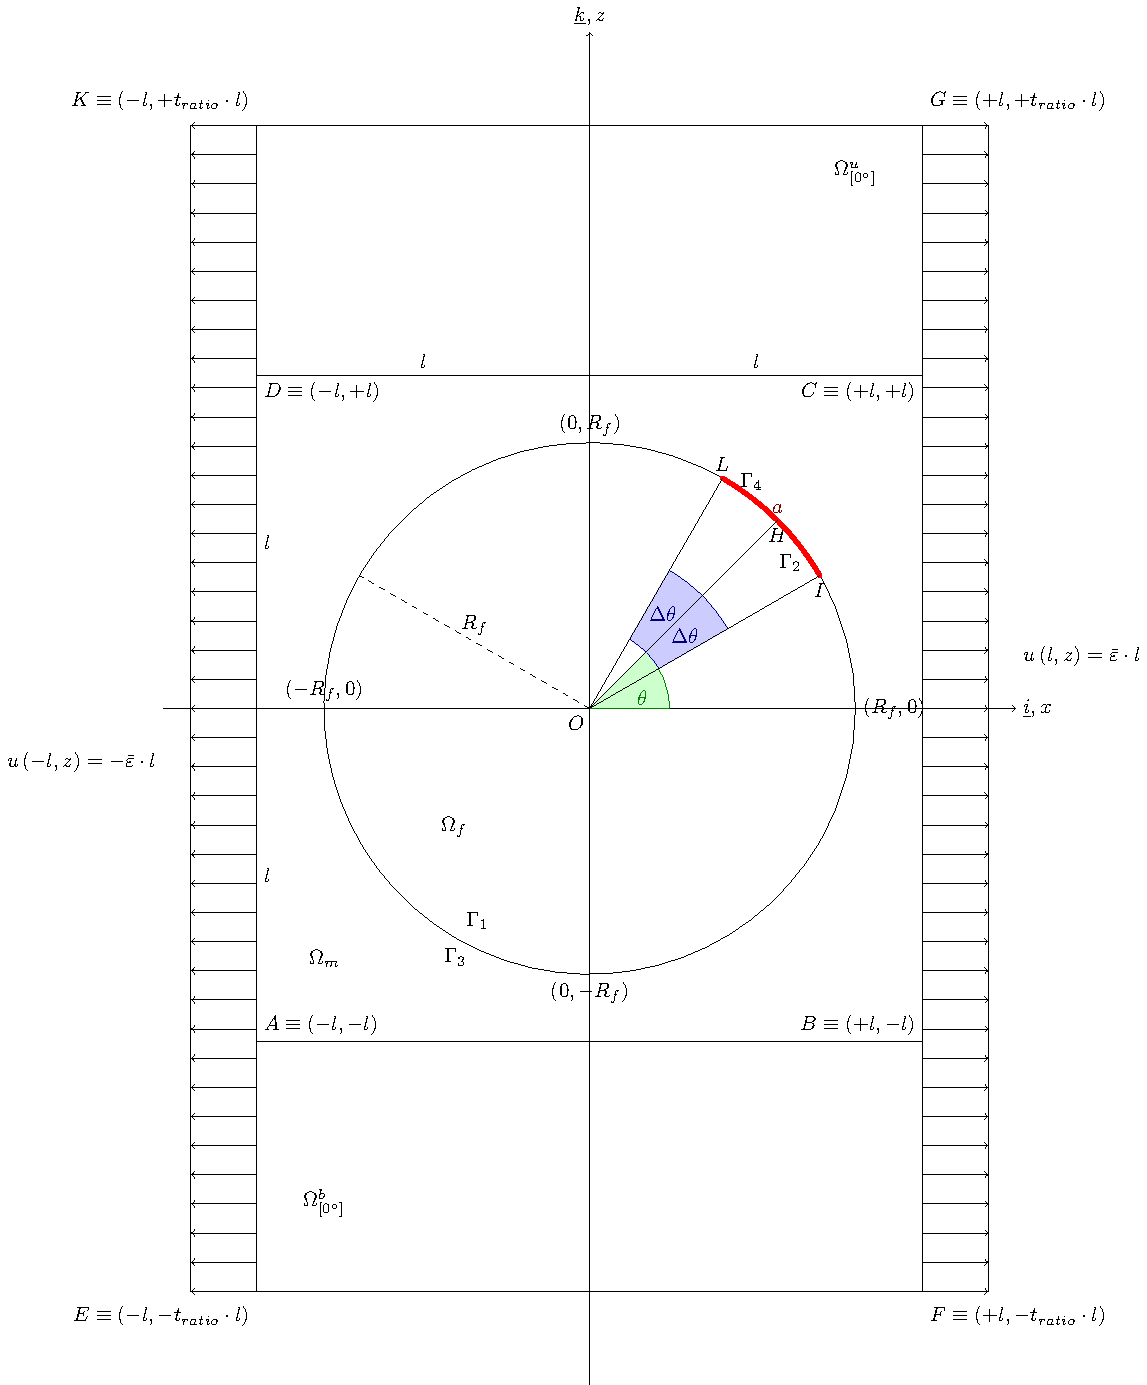
\includegraphics[width=\columnwidth]{boundedRVE_cc.pdf}
\end{figure}
\end{column}
\begin{column}{0.15\textwidth}
\begin{figure}[!h]
\centering
   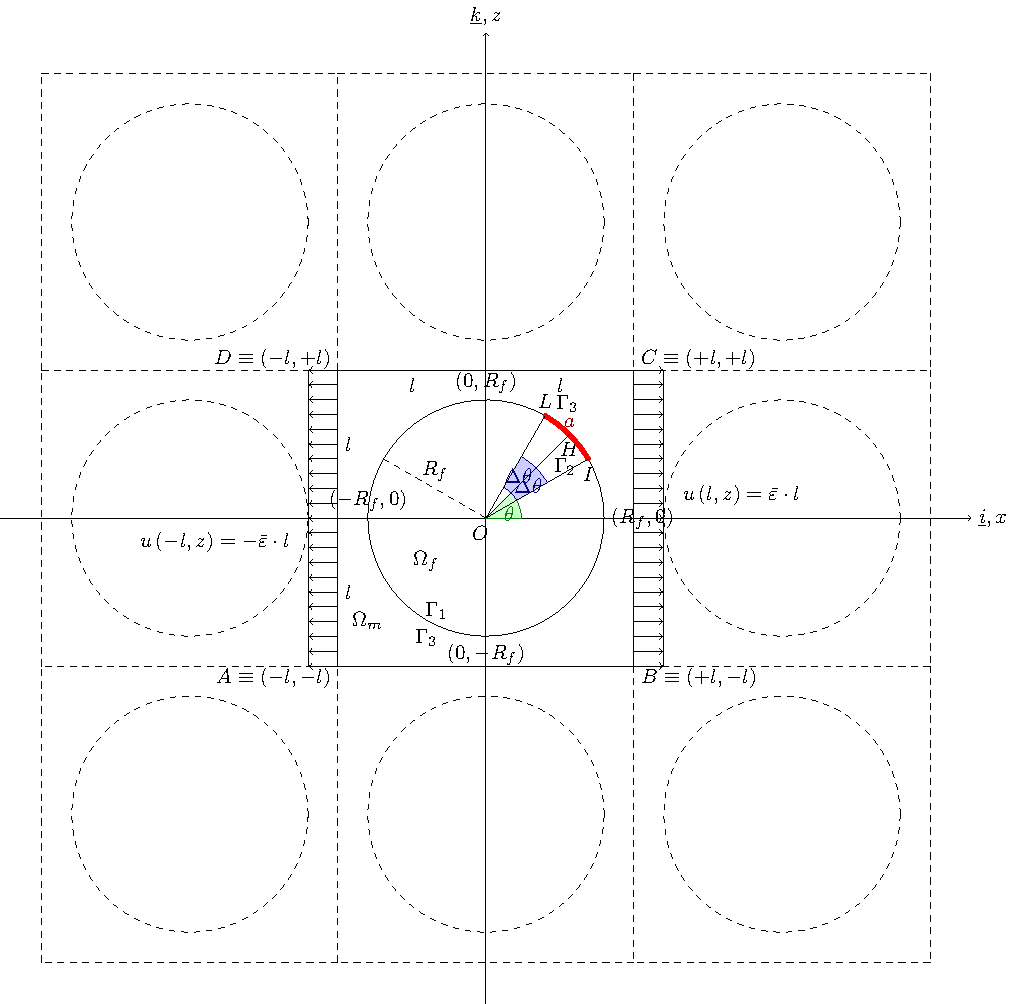
\includegraphics[width=\columnwidth]{periodicRVE_cc.pdf}
\end{figure}
\end{column}
\begin{column}{0.2\textwidth}  %%<--- here
    \begin{center}
\captionsetup[subfigure]{labelformat=empty}
\begin{figure}[!h]
\centering
    \subfloat[\bfseries VCCT: $G_{I}=\frac{Z_{C}\Delta w_{C}}{2B\Delta a}\quad G_{II}=\frac{X_{C}\Delta u_{C}}{2B\Delta a}$]{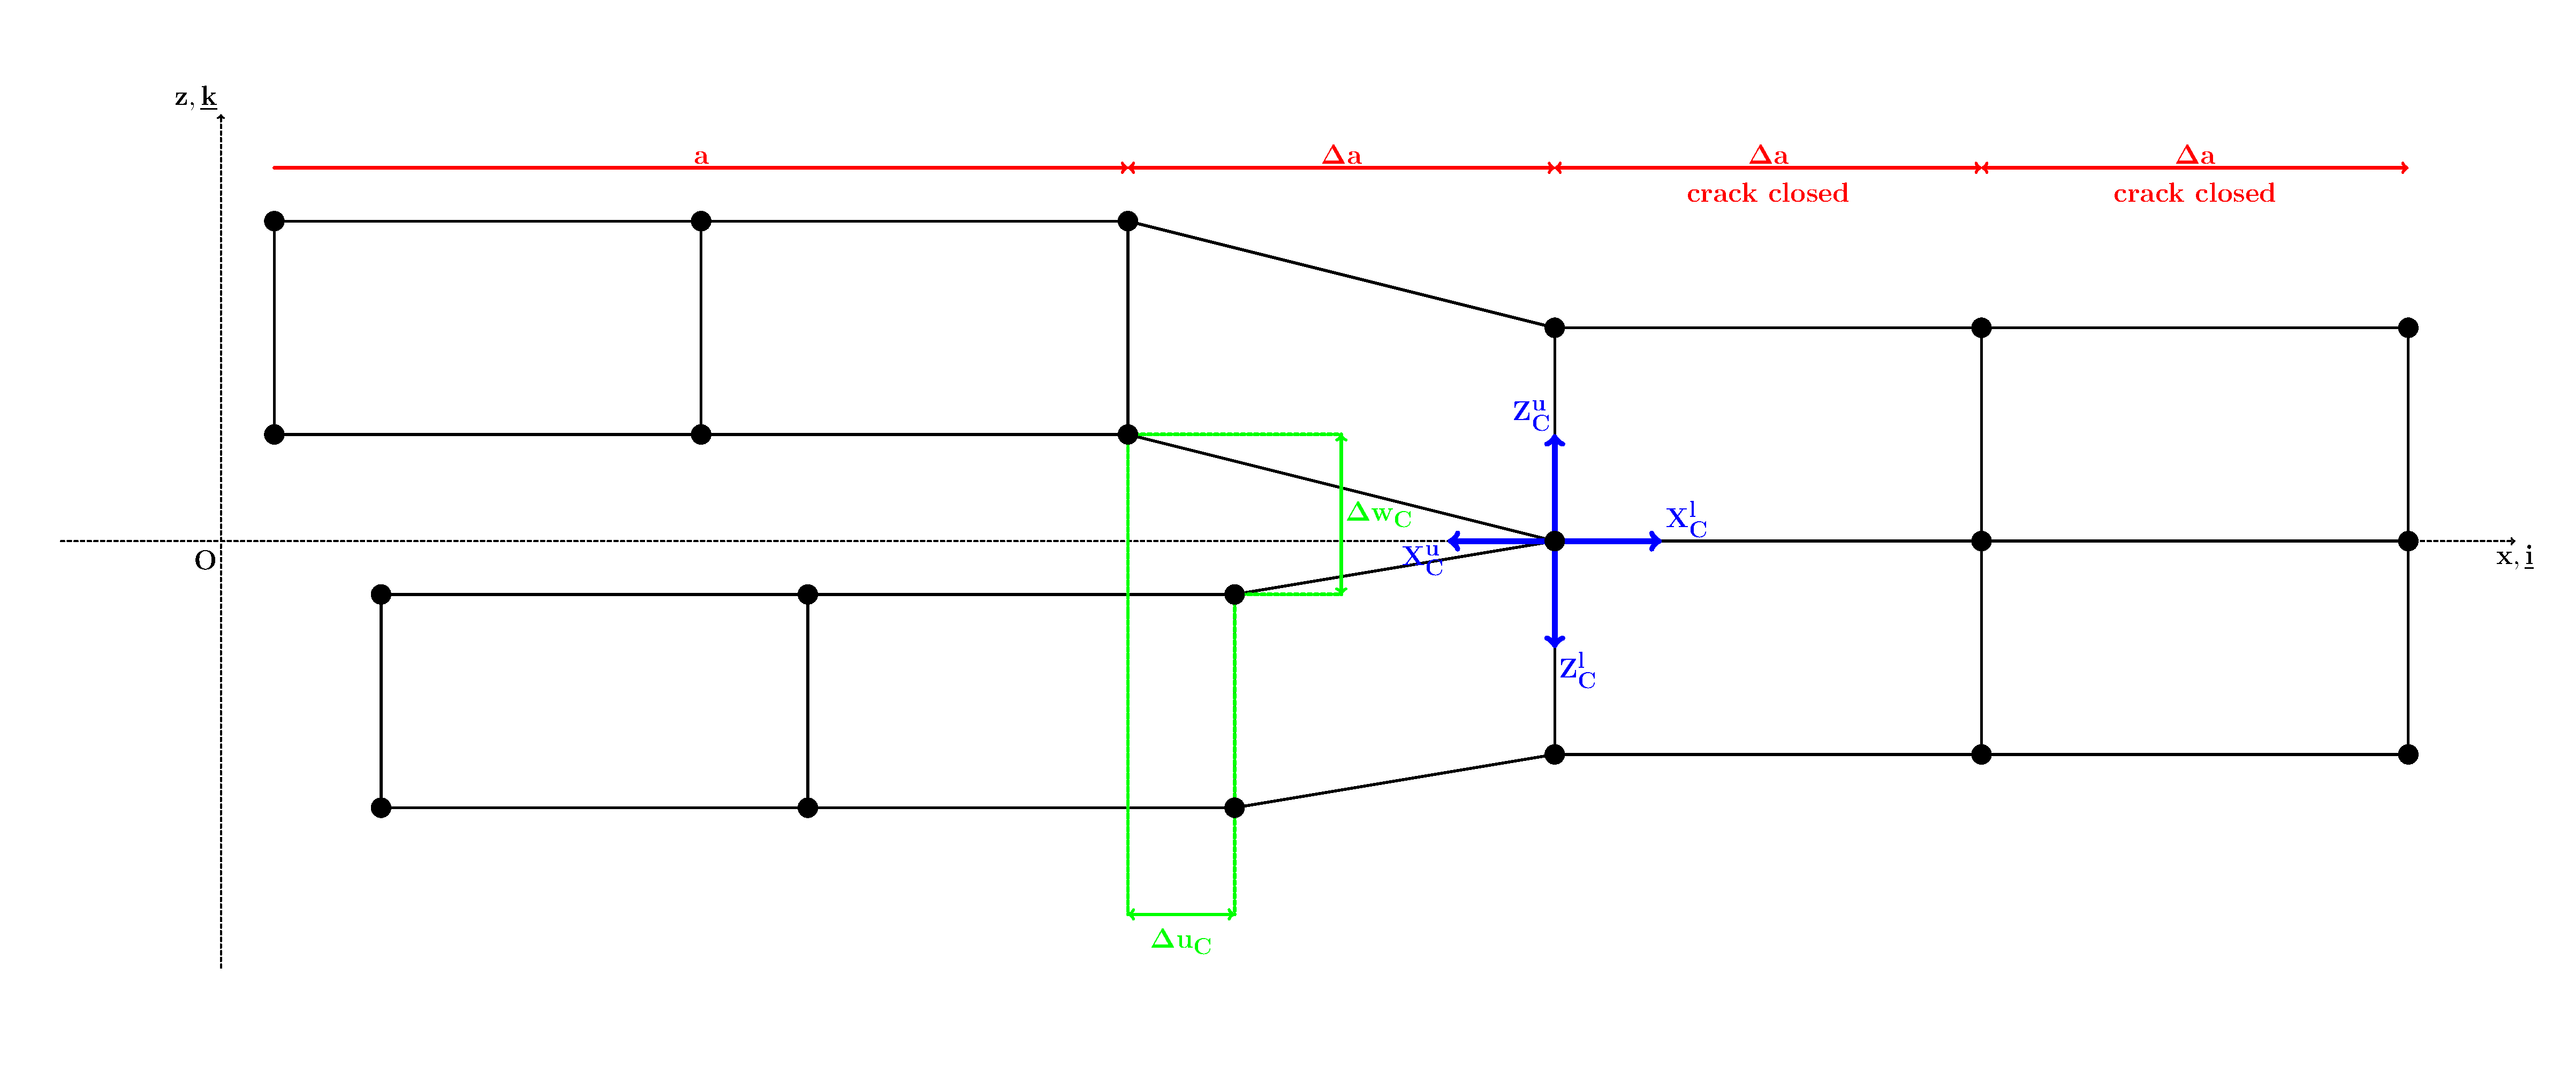
\includegraphics[width=\columnwidth]{VCCT.pdf}}\\
\subfloat[\bfseries J-Integral: $J_{i}=\lim_{\varepsilon\to 0}\int_{\Gamma_{\varepsilon}}\left(W\left(\Gamma\right)n_{i}-n_{j}\sigma_{jk}\frac{\partial u_{k}\left(\Gamma,x_{i}\right)}{\partial x_{i}}\right)d\Gamma$]{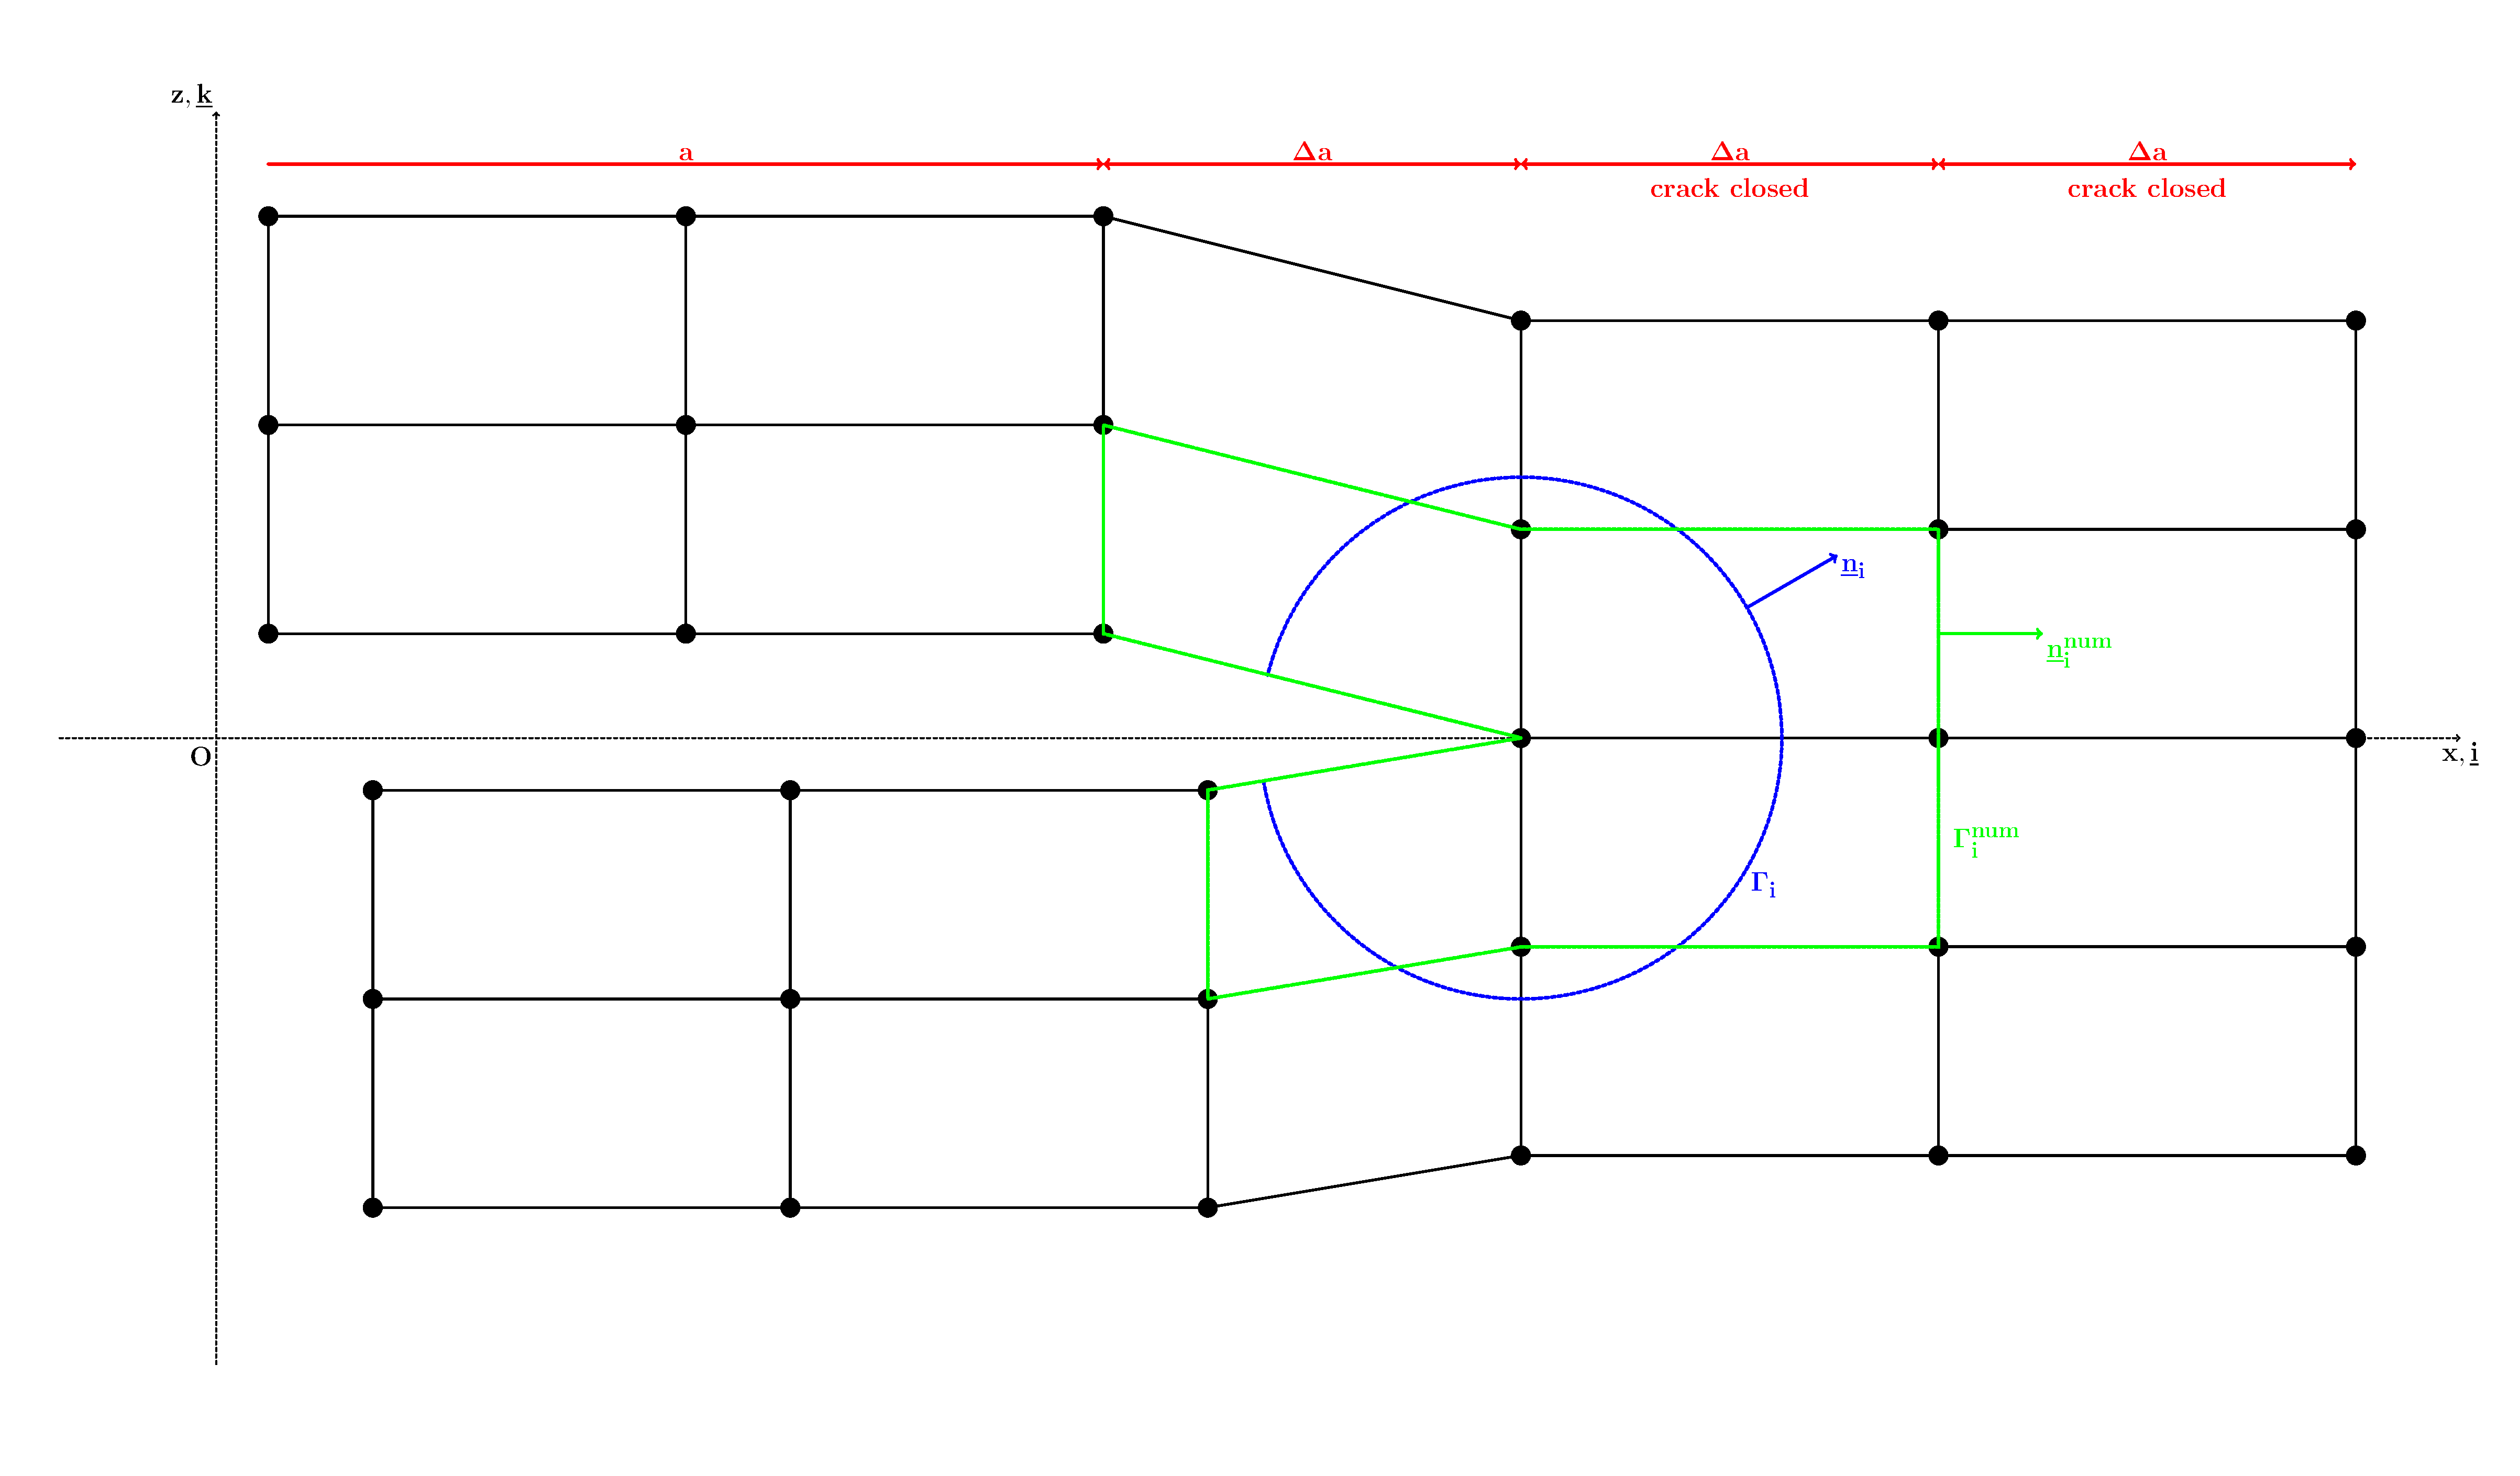
\includegraphics[width=\columnwidth]{J-integral.pdf}}
\end{figure}
     \end{center}
\end{column}
\end{columns}
\end{exampleblock}
\end{minipage}
\end{center}

\begin{center}
\begin{minipage}{\textwidth}
\begin{exampleblock}{\rule[-0.6ex]{0pt}{50pt}\centering\LARGE Preliminary Results \& Validation}
\begin{columns}
\begin{column}{0.25\textwidth}
\captionsetup[subfigure]{labelformat=empty}
\begin{figure}[!h]
\centering
   \subfloat[$\Delta\theta=15^{\circ},\delta=0.4^{\circ},VF_{f}=0.001,\frac{l}{R_{f}}\approx28$]{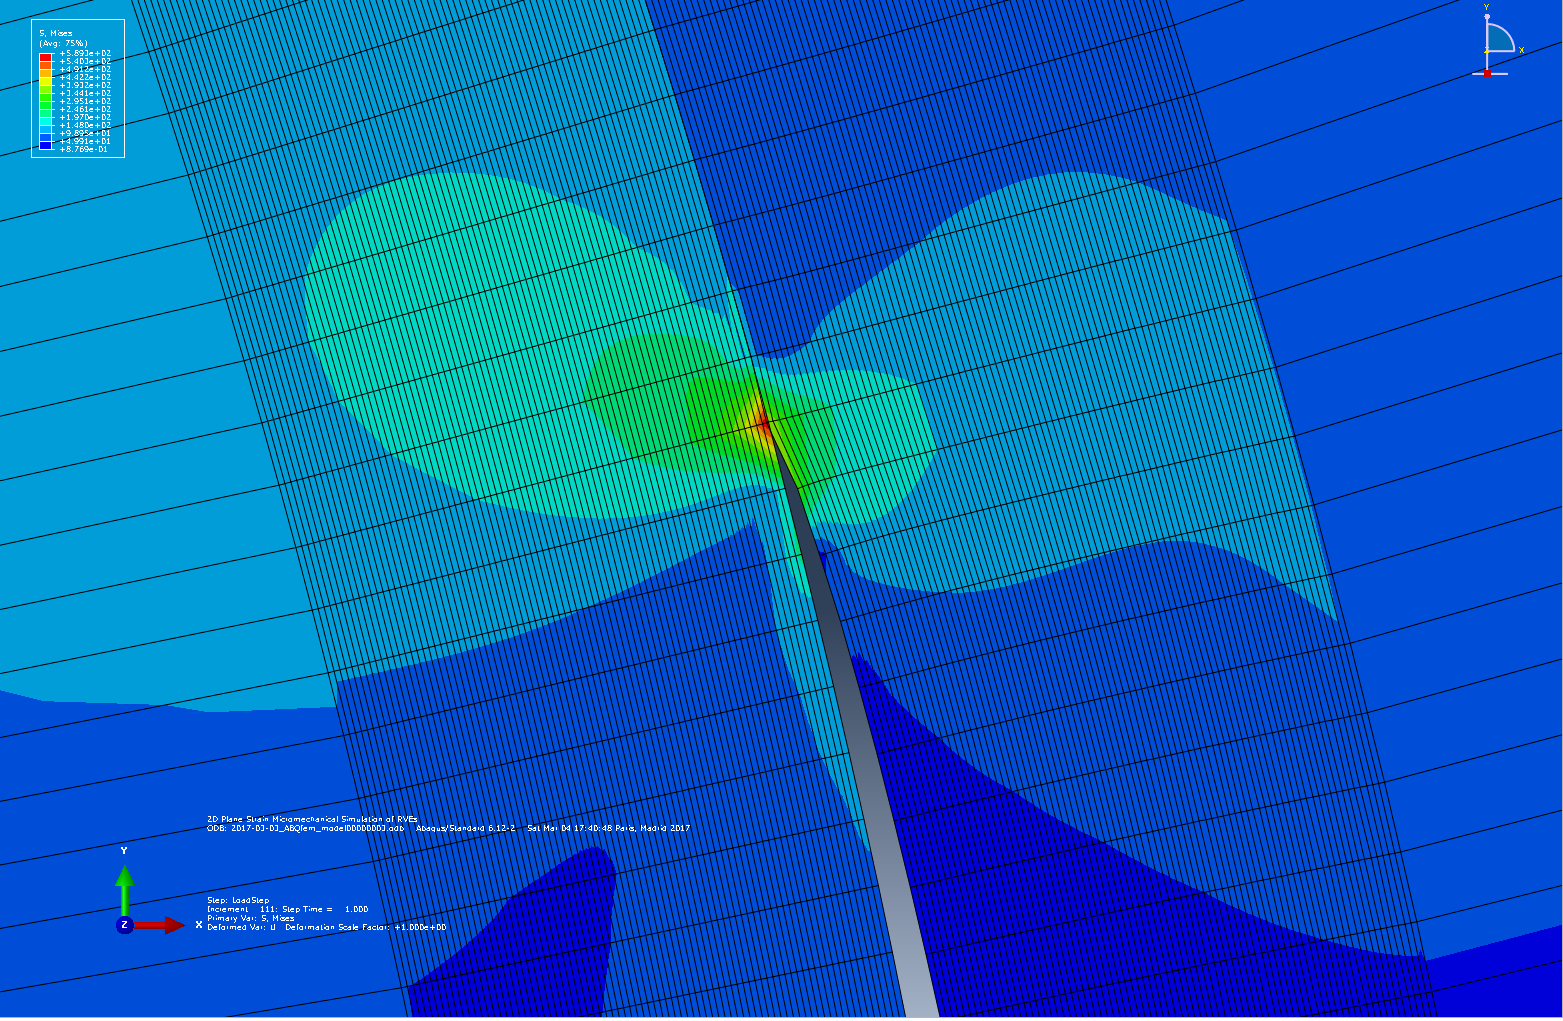
\includegraphics[width=0.9\columnwidth,height=0.11\textheight]{abq-crack-theta-15.png}}\\
\subfloat[$\Delta\theta=100^{\circ},\delta=0.4^{\circ},VF_{f}=0.001,\frac{l}{R_{f}}\approx28$]{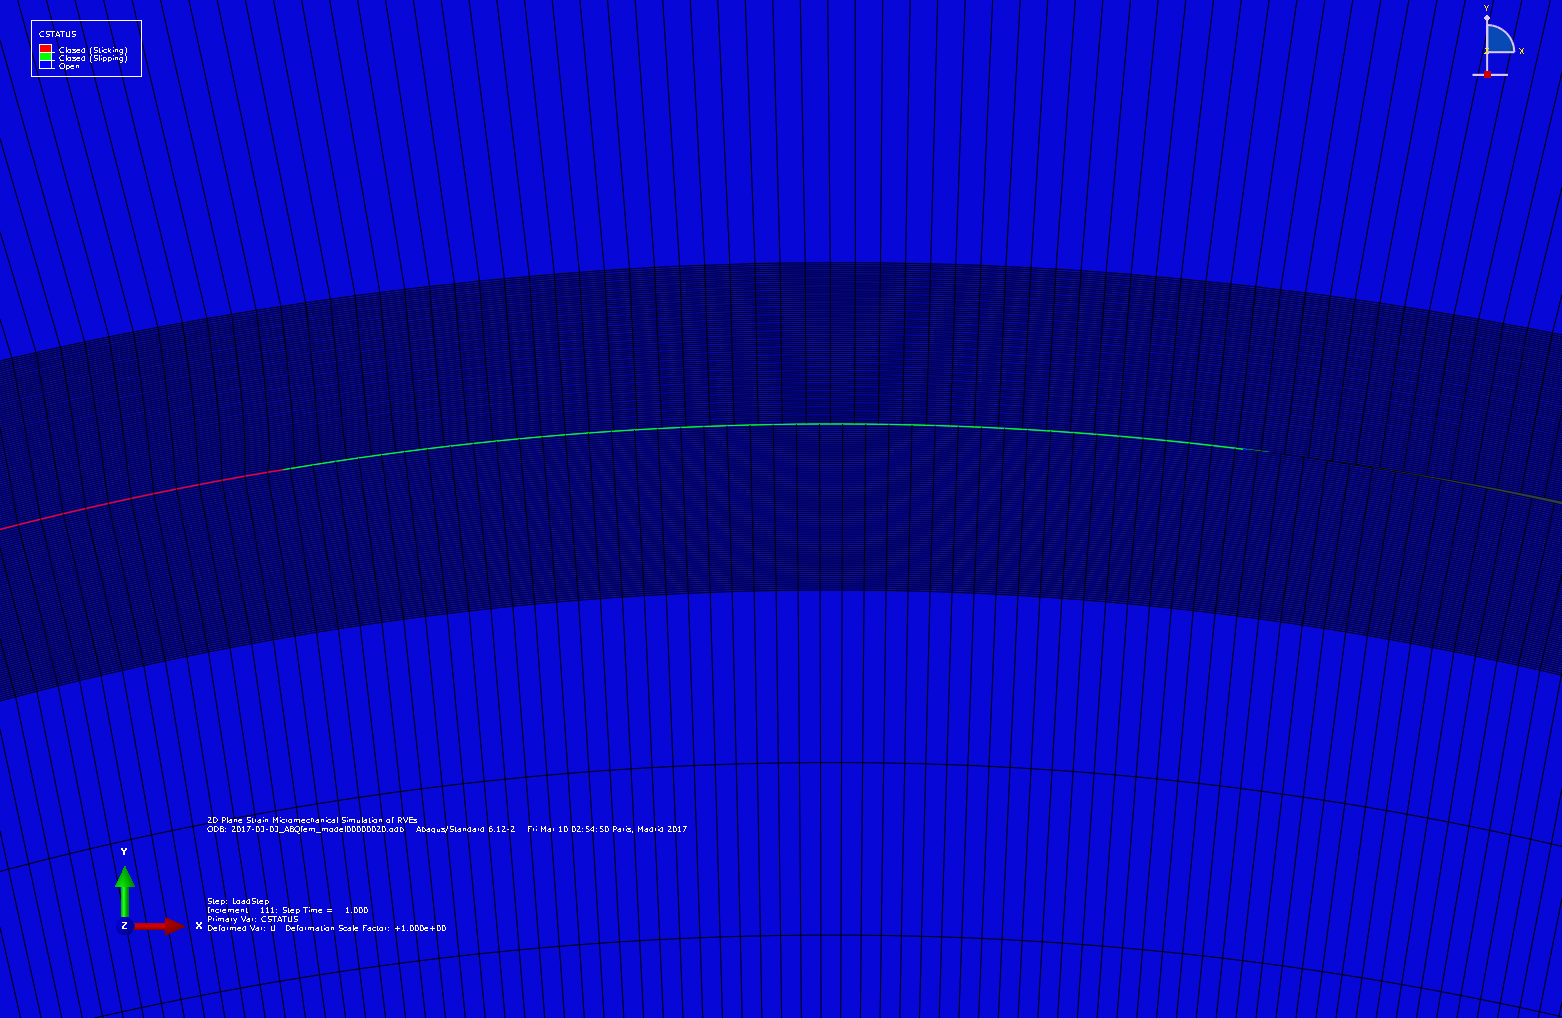
\includegraphics[width=0.9\columnwidth,height=0.11\textheight]{abq-crack-theta-100.png}}
\end{figure}
\end{column}
\begin{column}{0.375\textwidth}  %%<--- here
    \begin{center}
\captionsetup[subfigure]{labelformat=empty}
\begin{figure}[!h]
\centering
 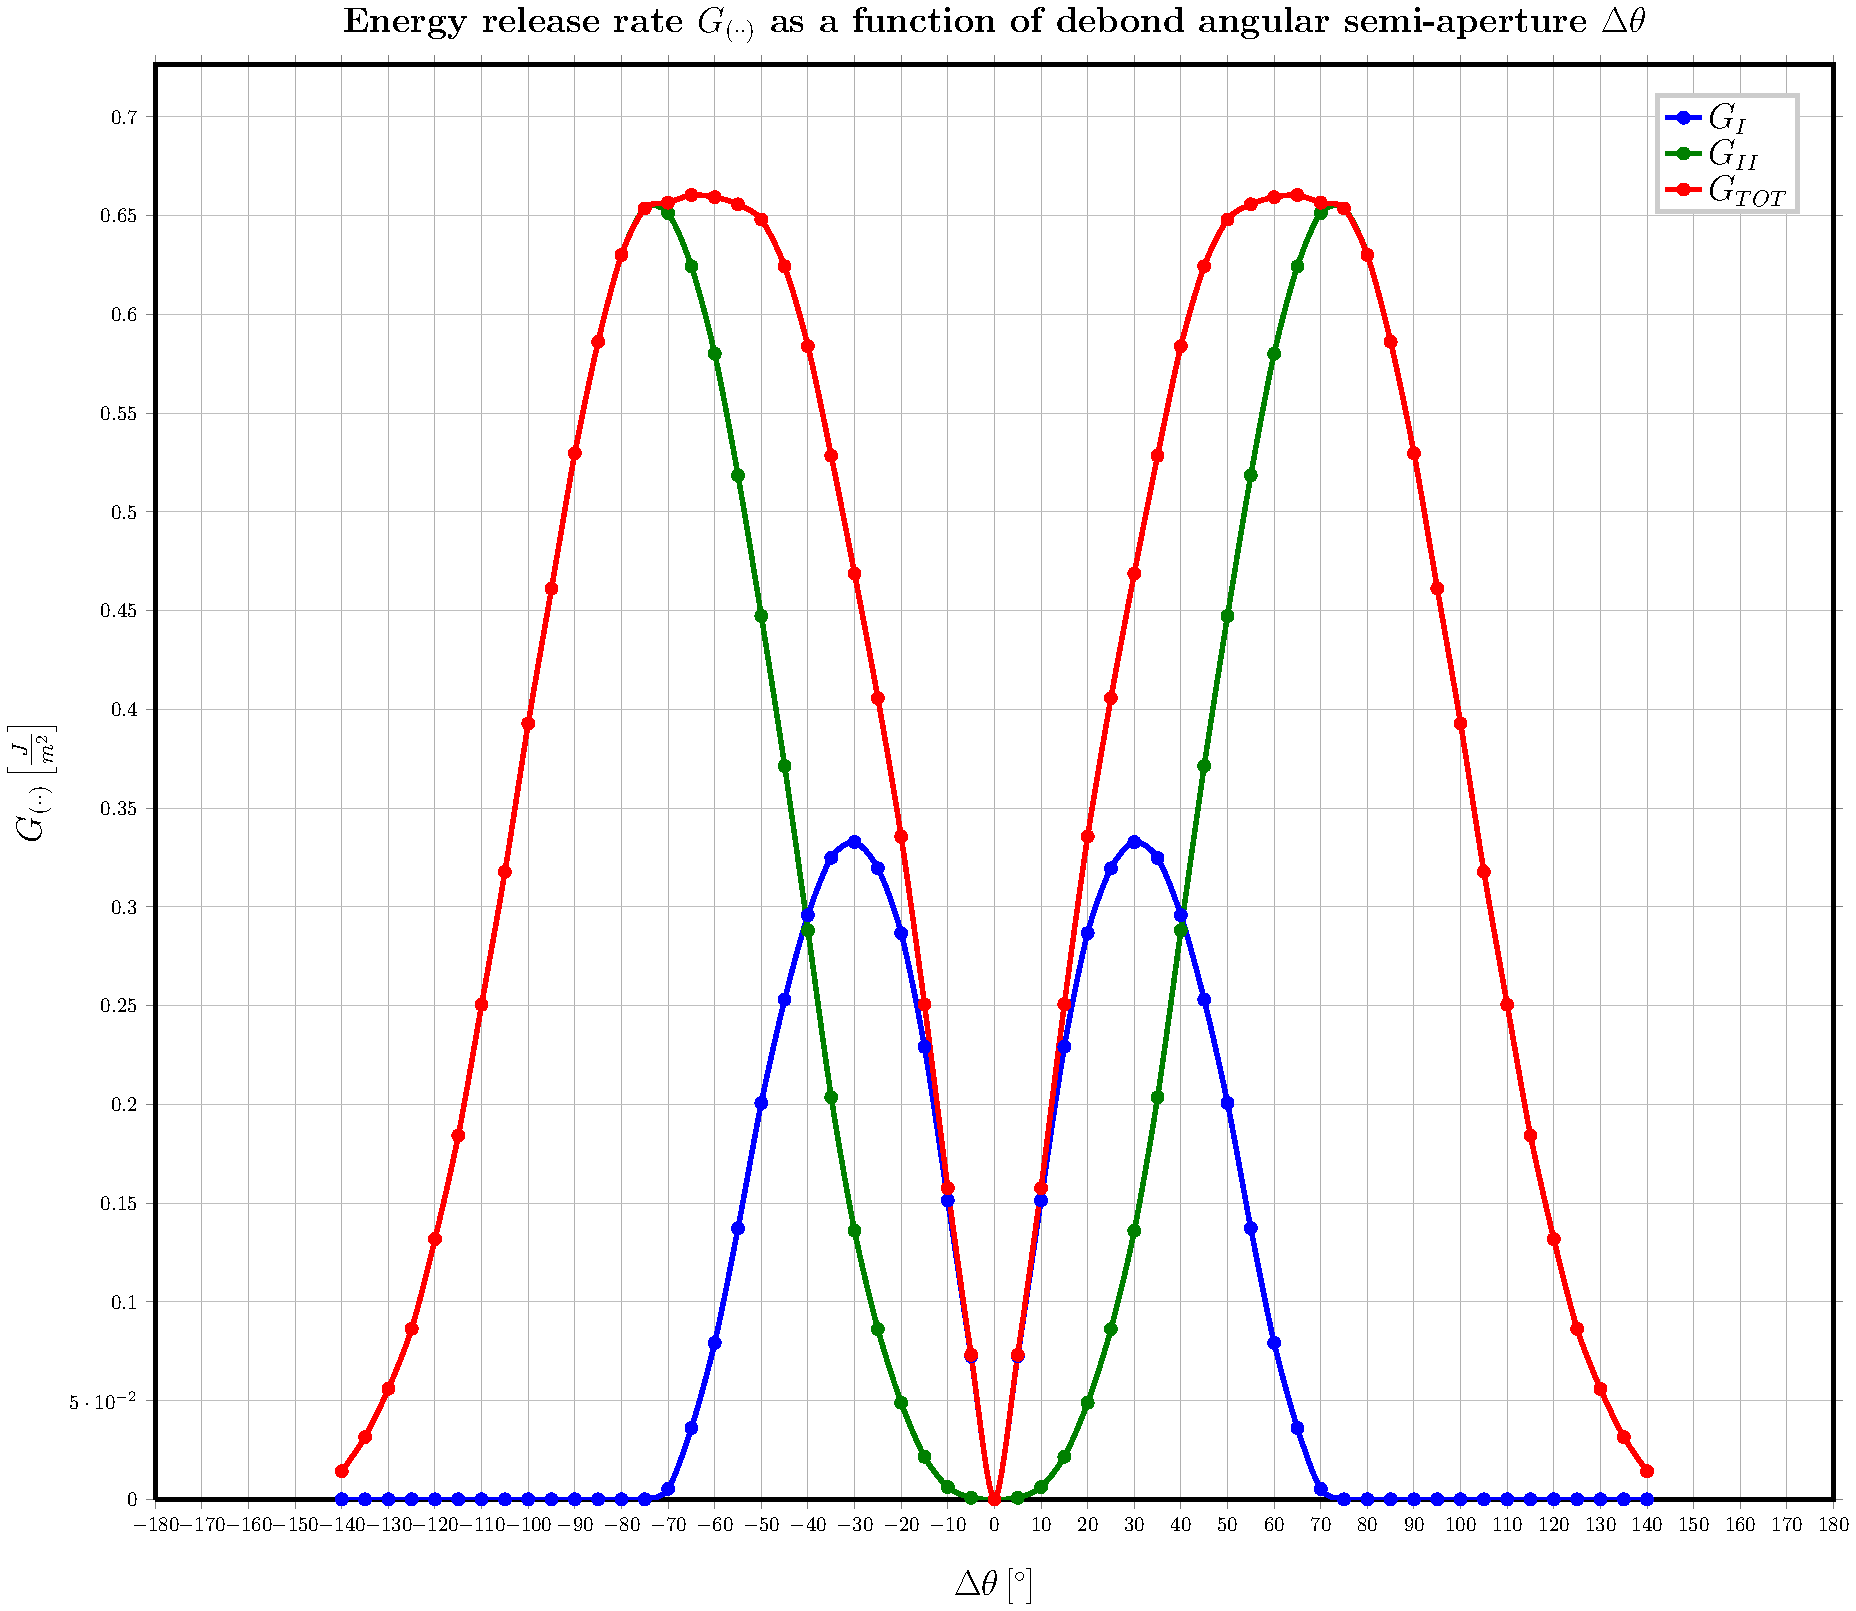
\includegraphics[width=0.9\columnwidth]{2017-03-03_AbqRunSummary_Gs.pdf}
 \caption{$\delta=0.4^{\circ},VF_{f}=0.001,\frac{l}{R_{f}}\approx28$}
\end{figure}
     \end{center}
\end{column}
\begin{column}{0.375\textwidth}  %%<--- here
    \begin{center}
\begin{figure}[!h]
\centering
     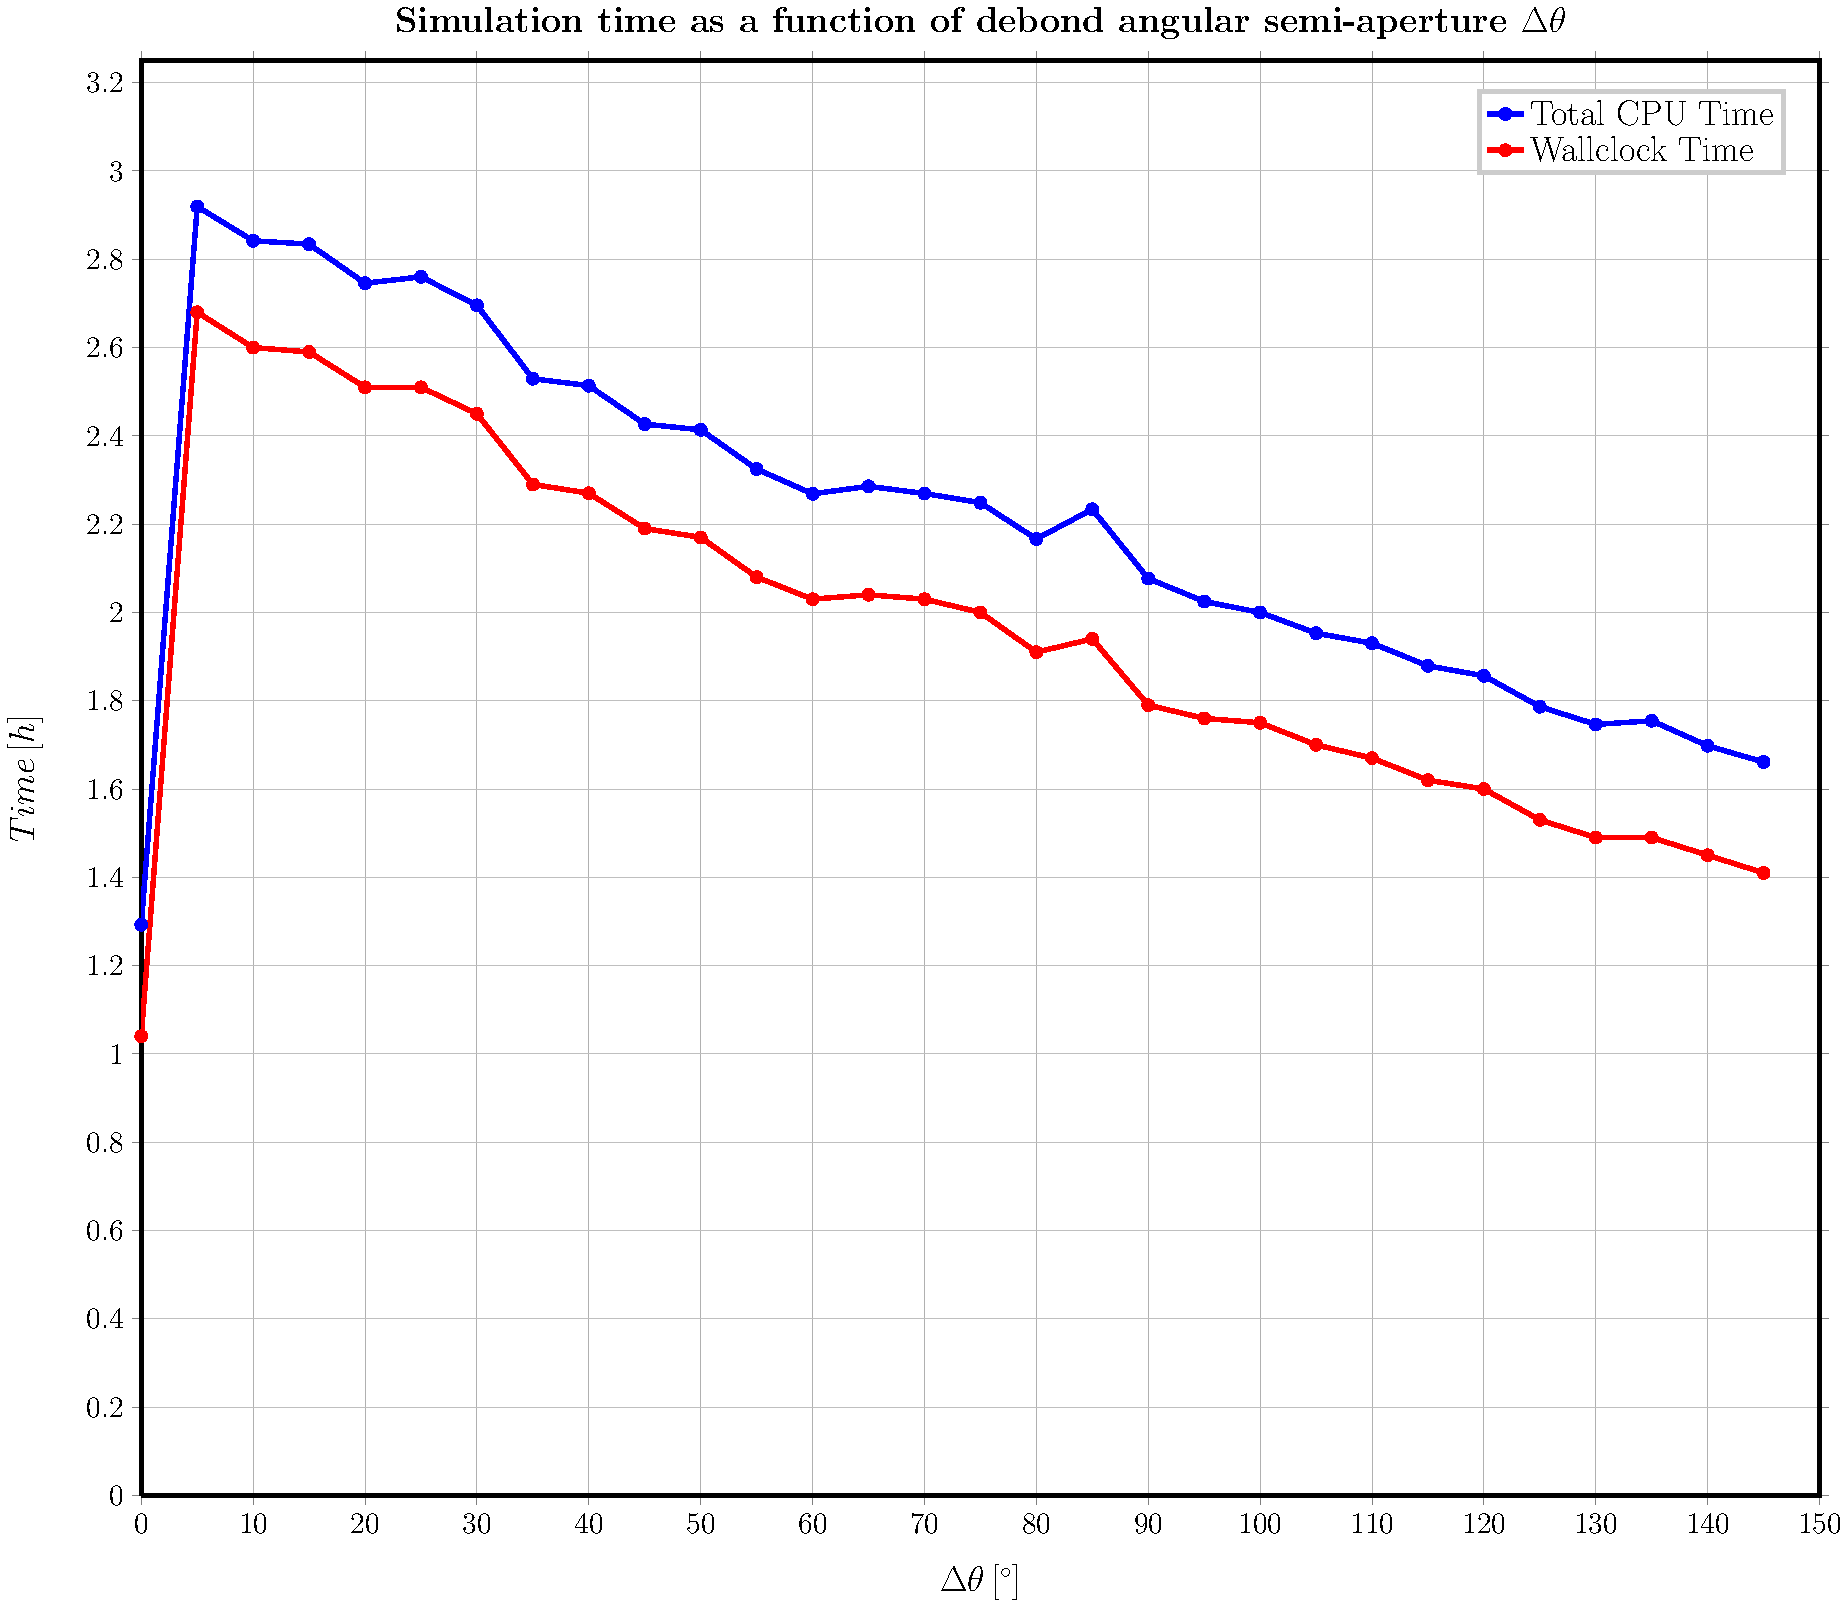
\includegraphics[width=0.9\columnwidth]{cpus-time.pdf}
 \caption{$\delta=0.4^{\circ},VF_{f}=0.001,\frac{l}{R_{f}}\approx28$}
\end{figure}
     \end{center}
\end{column}
\end{columns}
\end{exampleblock}
\end{minipage}
\end{center}

\begin{center}
	\begin{minipage}{\textwidth}
		\begin{alertblock}{\rule[-0.6ex]{0pt}{50pt}\centering\LARGE Conclusions \& Perspectives}
			\begin{columns}
				\begin{column}{0.475\textwidth}
   					 \begin{center}
						\textbf{What has been accomplished?}\\[10pt]
							\begin{itemize}
    								\item 2D micromechanical models have been developed to investigate crack initiation in thin ply laminates
								\item A numerical procedure has been devised and implemented to automatize the creation of FEM models
								\item Validation for $VF_{f}\to 0$ (matrix dominated RVE) with respect to previous literature [4, 5]
							\end{itemize}
   					\end{center}
				\end{column}
				\begin{column}{0.475\textwidth}  %%<--- here
   					\begin{center}
						\textbf{What's next?}\\[10pt]
						\begin{itemize}
    							\item Investigate the dependence on $VF_{f}$, $t_{ply}$, $t_{ply}/t_{bounding\ plies}$ and different material systems
							\item Study numerical performances with respect to model's parameters
							\item Repeat for different RVEs and compare
						\end{itemize}
   					\end{center}
				\end{column}
			\end{columns}
		\end{alertblock}
	\end{minipage}
\end{center}


\setbeamercolor{block title}{fg=black,bg=gray!40}
\setbeamercolor{block body}{fg=black,bg=gray!10}
\newsavebox{\squaredblocktext}
\setbeamertemplate{block begin}{
    \par\vskip\medskipamount%
    \makebox[\dimexpr\textwidth-1.5ex\relax][l]{%
        \begin{beamercolorbox}[colsep*=.75ex]{block title}
            \usebeamerfont*{block title}\insertblocktitle%
        \end{beamercolorbox}}%
        \begin{lrbox}{\squaredblocktext}%
            \begin{minipage}[t]{\textwidth}%
                \ifbeamercolorempty[bg]{block body}{\vskip-.25ex}{\vskip-.75ex}\vbox{}%
}

\setbeamertemplate{block end}{
            \end{minipage}%
        \end{lrbox}%
        {\parskip0pt\par}%
        \ifbeamercolorempty[bg]{block title}{}
        {\ifbeamercolorempty[bg]{block body}{}{\nointerlineskip\vskip-0.5pt}}%
        \usebeamerfont{block body}%
        \makebox[\dimexpr\textwidth-1.5ex\relax][l]{%
        \begin{beamercolorbox}[colsep*=.75ex,vmode]{block body}%
            \usebox{\squaredblocktext}
        \end{beamercolorbox}%
    }\vskip\smallskipamount%
}

\begin{center}
\begin{minipage}{\textwidth}
\begin{columns}[totalwidth=0.925\textwidth]
%\begin{column}{0.05\linewidth}
%\end{column}
\begin{column}{0.45\textwidth}
%\begin{center}
\begin{block}{\rule[-0.6ex]{0pt}{50pt}\centering Acknowledgements}
\centering\scriptsize The support of the European Commission through the Erasmus Mundus Programme is thankfully aknowledged.
\end{block}
%\end{center}
\end{column}
\begin{column}{0.45\textwidth}
%\begin{center}
\begin{block}{\rule[-0.6ex]{0pt}{50pt}\centering References}
\centering
\tiny
\begin{enumerate}
\item[{[}1{]}] NTPT makes world's thinnest prepeg even thinner. (2017, February 10). Retrieved from http://www.thinplytechnology.com/news-159-ntpta-makes-world-s-thinnest-prepreg-even-thinner
\item[{[}2{]}] oXeon TECHNOLOGIES. (2017, February 10). Retrieved from http://oxeon.se/technologies/
\item[{[}3{]}] Donald L. Flaggs, Murat H. Kural; Experimental Determination of the In Situ Transverse Lamina Strength in Graphite/Epoxy Laminates.  Journal of Composite Materials, 1982; 16(2).
\item[{[}4{]}] Toya, M.; A crack along the interface of a circular inclusion embedded in an infinite solid. Journal of the Mechanics and Physics of Solids, 1974; 22(5), pp. 325-348.
\item[{[}5{]}] Par\'is, F., Cano, J., and Varna, J.; The fiber-matrix interface crack - a numerical analysis using boundary elements. Int. J. Fract., 1990; 82(1), pp. 11-29.
\end{enumerate}
\end{block}
%\end{center}
\end{column}
\end{columns}
\end{minipage}
\end{center}

\end{frame}

\end{document}